\chapter{Sperimentazione}
\label{chap:impl}

In questo capitolo viene discussa l'implementazione e l'applicazione delle metriche di Model Selection e delle tecniche di Rank Aggregation. Infine viene proposta una valutazione su dataset di benchmark e quello di SKF.

Riassumendo, questo capitolo si dividerà in:
\begin{enumerate}
	\item Definizione e implementazione delle metriche surrogate per il Model Selection e delle tecniche di Rank Aggregation
	\item Valutazione su dataset benchmark
	\item Valutazione su SKF
\end{enumerate}


\section{Implementazione}
Come introdotto nel capitolo \ref{chap:modelselection}, il task da risolvere é l'implementazione di un metodo di Model Selection non supervisionato che scelga il modello o i modelli migliori dato un dataset. L'approccio scelto é stato quello di definire delle metriche "surrogate" che siano correlate con metriche supervisionate e che non richiedano etichette. Le metriche proposte sono indipendenti tra di loro ed é necessario usarne una come candidata oppure aggregarle secondo qualche criterio. Vengono quindi proposti diversi metodologie di Rank Aggregation. Uno schema rappresentante il flusso operazione é rappresentato in figura \ref{flow-scheme}.
\begin{figure}[t]
	\centering
	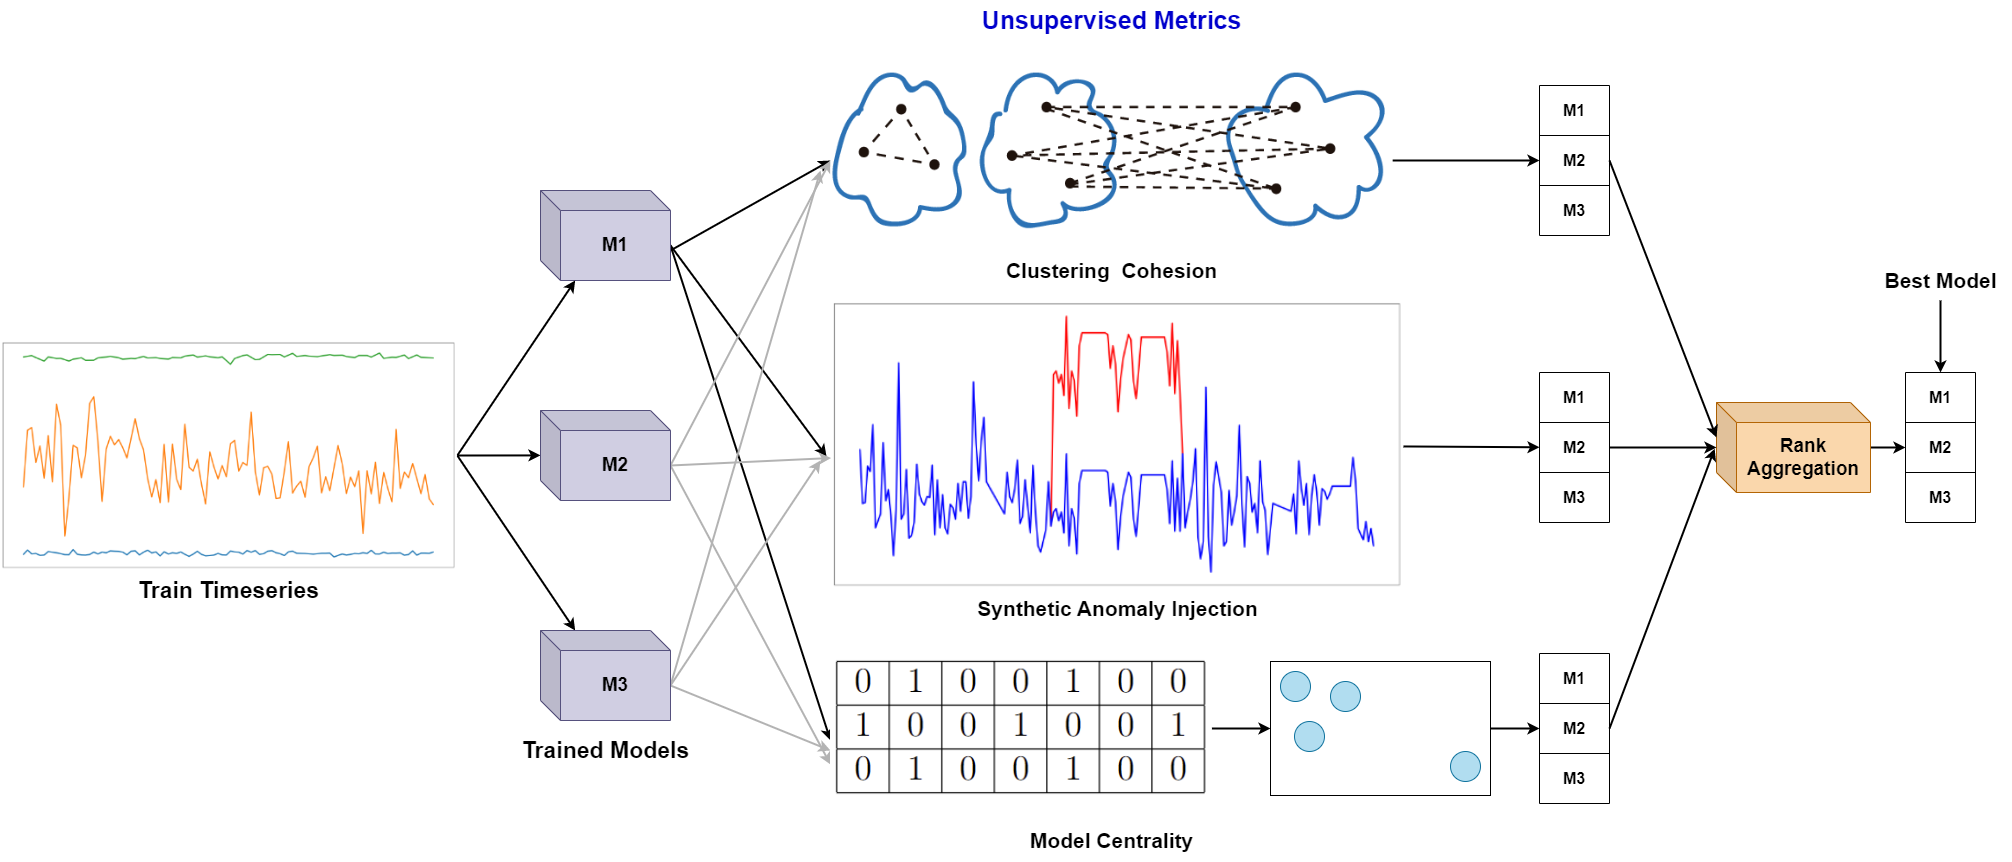
\includegraphics[width=14cm, scale=1]{images/model-selection-scheme}
	\caption{Flusso operazionale}
	\label{flow-scheme}
		
\end{figure}

\subsection{Metriche Surrogate}
Ogni metrica non supervisionata serve come misura della bontà di un modello e riduce il problema del Model Selection ad una selezione di quello con lo score più alto. 
Sono state identificate tre classi di metriche e vengono definite non supervisionate in quanto non richiedono etichette. Tuttavia, due di queste utilizzano internamente lo F1 Score, tipicamente utilizzato per la valutazione supervisionata; per evitare confusione viene quindi utilizzato il termine "surrogato".
Di seguito viene analizzata ogni classe di metriche surrogate. 


\subsubsection{Model Centrality}
\textit{Esiste una sola ground truth, quindi i modelli vicini a questa sono anch'essi vicini tra loro ed il modello più "centrale" è il migliore.}
Metodi basati sulla centralità hanno ottenuto successi recenti nel Model Selection e nell'Anomaly Detection. 
Per adottare quest'idea si é fatto uso di diverse tecniche che andassero a produrre delle classifiche nella quale i modelli con score più alto erano indicati come quelli più "centrali".
Sono state proposti 4 metodi per computare lo score di Model Centrality. Ognuna di queste riceve come input un set di $K$ modelli a cui é stato fatto training non supervisionato su un dataset di riferimento. 
\begin{itemize}
	\item \textbf{Round Robin}: dati i $K$ modelli, ognuno di questi viene selezionato a turno e le sue etichette prodotte vengono usate come ground truth per valutare le performance degli altri $K-1$ modelli. Infine viene prodotto un'unica classifica finale andando a calcolare la media delle performance di ogni modello rispetto alle $k-1$ iterazioni. 
	\item \textbf{Majority Vote} é il metodo più semplice per generare consenso: dati $K$ modelli e le loro etichette, viene generato un nuovo set di labels finale andando a prendere, per ogni sample, l'etichetta che riceve più voti. Questo nuovo set viene usato come ground truth per valutare i K modelli.
	\item \textbf{Sampling}: per ogni sample all'interno del dataset viene scelto in maniera casuale un modello da usare per estrarne l'etichetta. Viene quindi prodotto un nuovo set di labels da usare come ground truth per valutare i K modelli.
	\item \textbf{Score Correlation}: questo metodo utilizza gli score prodotti da ogni modello, dove lo score, al contrario delle etichette, rappresenta un valore direttamente proporzionale alla probabilità che quel sample sia anomalo. Inizialmente vengono calcolati i ranking di posizione per ognuno di questi set di score: Sia $Ok(i)$ il rank del sample $i$ secondo gli score prodotti dal modello K. Viene poi definita la distanza dal modello $Ak$ al modello $Al$ come la distanza di Kendall, ovvero il numero di disaccordi per ogni possibile coppia, tra i rank di posizione dei due modelli. Infine viene misurata la centralità di un modello come la distanza media rispetto a tutti gli altri modelli.
\end{itemize}

Ognuna di questi metodi produce un ranking finale per cui i modelli con lo score più alto sono quelli più centrali. In particolare i metodi Round Robin, Majority Vote e Sampling che generano un set di etichette pseudo reali, utilizzano lo F1 Score per valutare ogni modello rispetto a questo set.

Questa metrica surrogata non é perfetta, mentre funziona bene quando i modelli candidati sono tutti sufficientemente buoni da un punto di vista delle performance; nel caso siano presenti un numero relativamente alto di modelli "non buoni", questi potrebbero produrre risultati simili e formare un cluster che va di fatto a condizionare la centralità.
Nella parte della valutazione su dataset di benchmark verranno analizzate le performance di ognuna di queste 4 metodologie.


\subsubsection{Performance on Injected Synthetic Anomalies}
\textit{Un buon modello di Anomaly Detection si comporterà bene anche su dataset con anomalie iniettate sinteticamente}. Alcuni paper hanno precedentemente esplorato l'uso dell'iniezione di anomalie sintetiche per addestrare modelli di rilevamento delle anomalie. Attraverso questa metrica surrogata, viene estesa questa linea di ricerca valutando sistematicamente la capacità dell'algoritmo di Model Selection dopo aver iniettato diversi tipi di anomalie. Dato un dataset di input senza etichette, vengono iniettate casualmente anomalie. La posizione dell'anomalia iniettata viene trattata come un'etichetta pseudo-positiva, mentre il resto dei punti sono trattati come punti pseudo-negativi. 
Infine ogni modello viene valutato attraverso l'F1 Score rispetto alle pseudo-etichette.

Invece di affidarsi a modelli generativi complessi, é stato sviluppato un semplice algoritmo che inietta anomalie di diverso tipo andando prima ad analizzare il dataset ricevuto in input. I tipi di anomalie iniettate prese in considerazione sono 3 e sono visibili in figura \ref{tipi-anomalie}: 
\begin{figure}[t]
	\centering
	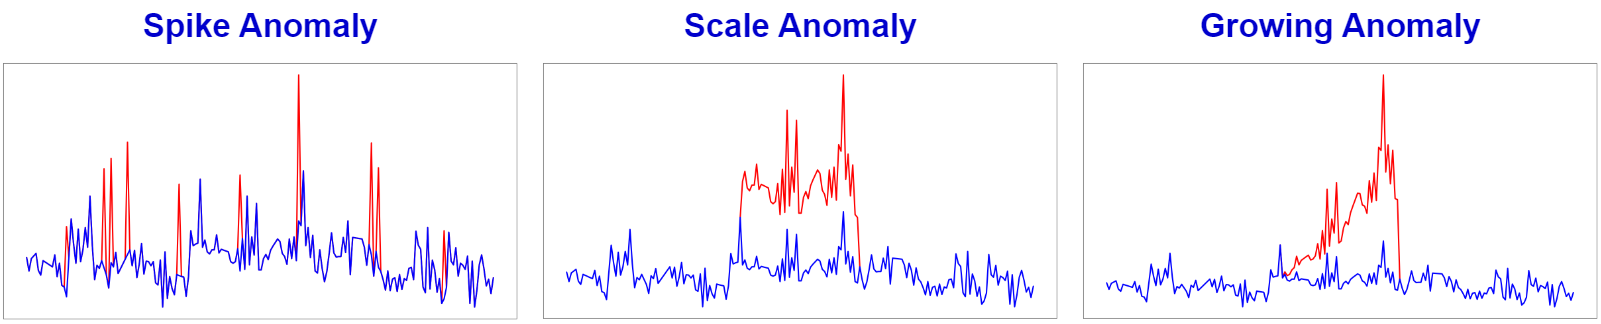
\includegraphics[width=14cm, scale=1]{images/anomalies}
	\caption{Tipologie di anomalie}
	\label{tipi-anomalie}
		
\end{figure}


\begin{enumerate}
	\item \textbf{Spike Anomaly} sono delle anomalie a punto in cui il valore nel punto si discosta in maniera significativa rispetto all'intorno. Lo spike ha un magnitudo governato da una distribuzione \[s \approx N(1.5, 3) \]
	\item \textbf{Scale Anomalies} é un intervallo di punti anomali in cui il  valore medio dei punti al suo interno é significativamente più grande o più piccolo rispetto all'intorno. I dati vengono scalati \[ ts_a[i, start:end] = factor*ts[i, start:end]\] dove \textit{factor} segue sempre la distribuzione \(s \approx N(1.5, 3) \)
	\item \textbf{Growing Anomalies} é un intervallo di punti anomali in cui il valore di essi cresce o decresce linearmente nel tempo. I dati vengono modificati secondo \[ ts_a[i, start:end] = np.linspace(0, baseline, end-start) + ts[i, start:end] \] 
\end{enumerate}

Il numero di anomalie da iniettare viene calcolato sulla base del fattore di contaminazione associato ad un determinato dataset. Ad esempio, su un dataset con 10000 sample ed un fattore di contaminazione di 0.05, 500 anomalie saranno iniettate.
La posizione nella quale vengono iniettate le anomalie a spike viene scelta casualmente; invece per quanto riguarda le anomalie a scale e growing, vengono generati casualmente dei punti di inizio intervallo mentre la lunghezza di questi é predisposta a mano in base alla frequenza dei sample o alla dimensione del dataset.

Attraverso uno studio di correlazione fra le feature del dataset si é andanti a scoprire se due o più feature dovessero essere considerate insieme quando si aggiunge un'anomalia in un determinato punto. In un esempio pratico, se la feature della Pressione e quella del Flusso hanno una correlazione vicina a -1, quindi negativa, l'iniezione dell'anomalia prevede che una delle due feature vede il suo valore modificato verso l'alto mentre l'altro verso il basso. L'immagine \ref{feature-correlazioni} mostra un esempio di correlazioni positiva e negativa.
\begin{figure}[t]
	\centering
	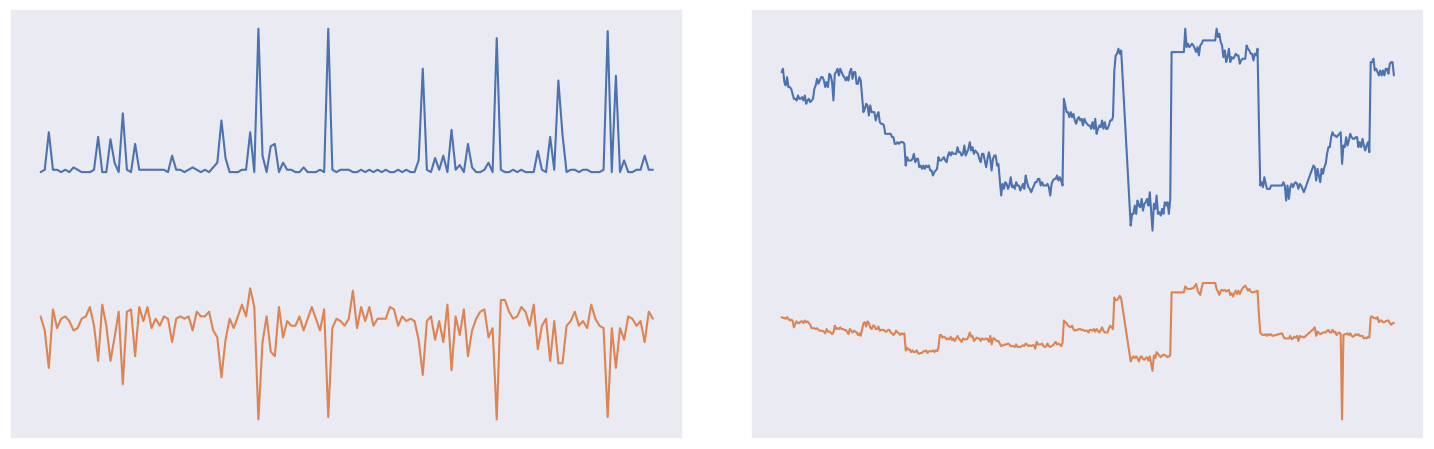
\includegraphics[width=14cm, scale=1]{images/corr}
	\caption{Correlazioni tra features}
	\label{feature-correlazioni}
		
\end{figure}

Utilizzando il coefficiente di Skew si va a vedere in che direzione portare l'anomalia: se verso il basso o verso l'alto. Feature con un right-skew avranno anomalie orientate verso l'alto, left-swek verso il basso mentre se non rientrano in nessuno dei due casi allora si generano anomalie casuali o verso il basso o verso l'alto.

Infine, calcolando l'indice di Kurt di definisce la probabilità con cui si sceglie una determinata feature per inserirvi un anomalia per ogni determinato punto. Un valore di Kurt più alto indica una probabilità di anomalie più alta per quella feature, questo per andare a favorire la generazione di anomalie per quelle feature che hanno una deviazione standard molto alta, al contrario di feature più "piatte" che cambiano di rado.


Le tipologie di anomalie sintetiche possono essere iniettate in modo esclusivo, ovvero generando N copie del dataset originario a cui si inseriscono una sola tipologia di anomalia per ognuna; oppure combinandole insieme in un unico dataset. 
Ognuno di questi dataset prodotti viene poi utilizzato per effettuare la valutazione sui modelli generando quindi N ranking differenti. Le performance di ognuno di questi metodi verranno valutate successivamente utilizzando lo F1-Score.

Il flusso di lavoro di questa metrica surrogata puo essere riassunta in questi step:
\begin{enumerate}
	\item Training dei modelli sul dataset originario
	\item Creazione di dataset modificati andando ad iniettare i diversi tipi di anomalie e producendo quindi le pseudo-etichette
	\item Valutazione dei modelli sui dataset modificati usando le pseudo-etichette come ground truth e F1 Score come metrica di valutazione.
\end{enumerate}


Questa procedura puo essere molto efficace ma non é esente da problemi: (1) le anomalie reali non vengono considerate e di conseguenza sono etichettate come pseudo-negative. Questo potrebbe portare a score falsati nel caso i modelli andassero a riconoscere prevalentemente solo le anomalie reali, che però nella fase di valutazione vengono visti come sample negativi. Infine (2) le tipologie di anomalie iniettate possono risultare molto differenti da quelle che sono le reali anomali, rischiando quindi di produrre score molto alti per certi modelli ma che nella realtà funzioneranno particolarmente male sul dataset originario.

\subsubsection{Clustering Cohesion}
\textit{Un buon modello riesce a trovare una buona separazione tra i punti normali ed i punti anomali}.
Nel contesto dei modelli non supervisionati, tecniche e metriche di valutazione inerenti al clustering sono molto efficaci quando non si hanno a disposizione le etichette. Misure di coesione tra i cluster prodotti da un modello sono indicatori di quanto quest'ultimo sia riuscito a separare efficacemente i dati.
All'interno del task dell'Anomaly Detection, le anomalie sono punti che di discostano in maniera significativa da un comportamento normale e di conseguenza avranno valori molto diversi rispetto al resto dei punti. Immaginando i punti considerati normali con un unico cluster, ci si aspetta che questi siano ben raggruppati insieme mentre i punti anomali sono sparsi o al più raggruppati in zone poco dense.
\begin{center}
	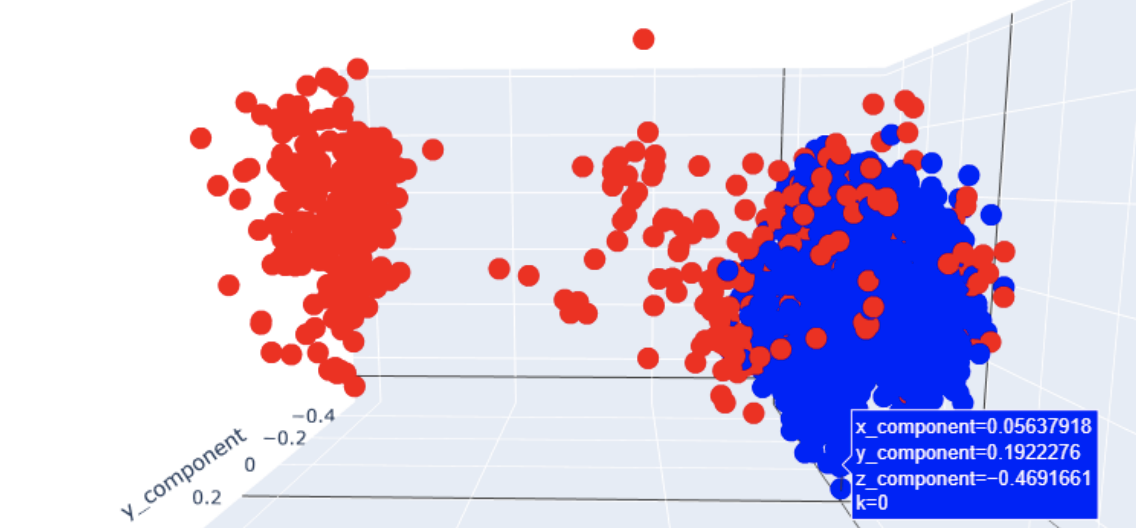
\includegraphics[width=12cm, scale=1]{images/plot-anomalies-normal}
    \captionsetup{type=figure}
	\captionof{figure}{Scatter plot dopo l'Anonaly Detection}
    \label{plot-anomalies-normal}
\end{center}
L'idea alla base di questa metrica surrogata é quindi quella di calcolare la coesione e separazione tra il cluster di punti normali e quello di punti anomali prodotti dalle etichette di un modello di Anomaly Detection. Più alto é questo score, più il modello riesce a separare questi dati e quindi puo essere considerato come un buon modello.
La metrica utilizzata é il Silhouette Score, ma non viene calcolata subito dopo aver ottenuto le etichette da un modello. Sono necessari prima alcuni passaggi di processamento del dato.
Immaginiamo di avere un dataset con due feature per la quale é possibile visualizzare graficamente i punti in un piano cartesiano. Idealmente i punti considerati normali formano un unico cluster denso, ma la stessa cosa non si puo dire per i punti anomali. 
Questi possono essere sparsi per il piano come se fossero rumore oppure possono formare cluster di piccole dimensioni, ma in ogni caso questi punti anomali hanno tutti la stessa etichetta (Figura \ref{plot-anomalies-normal}).
Il Silhouette Score calcolato assumendo solo etichette di valore 0 o 1 potrebbe risultare falsato proprio per il fatto che i punti sparsi contribuiscono in maniera negativa allora score.

La soluzione adottata é quella di applicare l'algoritmo di DBSCAN sui punti anomali, per formare quindi più cluster da questi e per scartare quei punti che vengono etichettati dall'algoritmo come rumore.
Prima di fare ciò però é necessario ridurre la dimensionalità dei dati per evitare il problema del "Curse Of Dimensionality", il quale afferma che in un dataset ad alta dimensionalità, la distanza tra i singoli punti é troppo alta per essere informativa.
Applicando quindi PCA per ridurre le dimensioni a 3, rende l'applicazione di DBSCAN più efficace. Come parametri sono stati usati $minsamples=dim \cdot 2$ e per quanto riguarda $eps$ é stato ricavato il valore usando l'Elbow Method.
Applicando quindi DBSCAN si ottengono i cluster per i punti anomali come mostrato in Figura \ref{plot-dbscan-anomalies}: i punti gialli sono considerati rumore, mentre il restante dei colori sono i cluster di punti anomali.

\begin{center}
	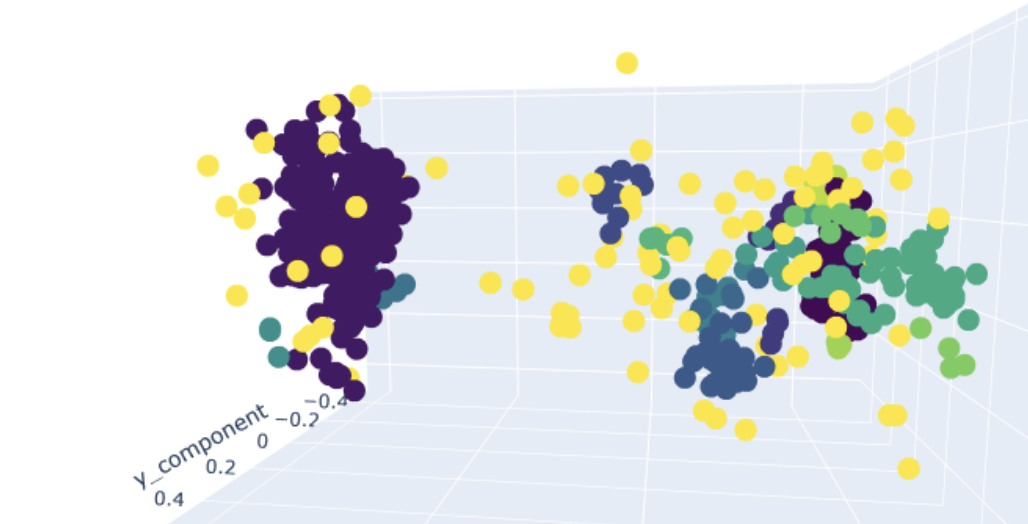
\includegraphics[width=12cm, scale=1]{images/plot-dbscan-anomalies}
    \captionsetup{type=figure}
	\captionof{figure}{Scatter plot dopo DBSCAN sulle anomalie}
    \label{plot-dbscan-anomalies}
\end{center}

Infine viene calcolato il Silhouette Score su questi, tenendo anche in considerazione il cluster di punti normali originario. Questa procedura viene poi applicata su ogni modello per andare a produrre un ranking finale.

Questa metrica surrogata puo funzionare particolarmente bene quando l'autocorrelazione di una serie temporale é relativamente bassa, quindi stazionaria, e quindi i punti sono quasi indipendenti tra di loro. Le anomalie a punto così come le anomalie collettive sono identificate con più precisione rispetto alle anomalie contestuali. Infatti, per definizione, i primi due tipi rappresentano punti molto distanti rispetto all'insieme totale, mentre il terzo tipo rappresenta punti distanti rispetto ad un intorno ma che potrebbero essere valutati normali rispetto ad altri intervalli, risultando quindi con più probabilità nel cluster di punti normali.
\subsection{Rank Aggregation}
Nel capitolo \ref{chap:modelselection} é stata fatta una panoramica su Rank Aggregation, vediamo ora quali tecniche sono state implementate. Un'analisi sulle performance di ognuno sarà svolta nelle sezioni successive.
Ognuno di questi metodi riceve in input un set di ranking, ognuno prodotto da una metrica surrogata diversa, ed in output viene generato un'unica classifica finale.
Nel caso delle metriche surrogate Model Centrality e Performance on Injected Synthetic Anomalies, il ranking prodotto si basa sul F1 Score; mentre per Clustering Cohesion sul Silhouette Score.
\subsubsection{Kemeny-Young}
È il metodo di Rank Aggregation ottimale in quanto ottimizza la funzione oggetto come definito nel capitolo \ref{chap:modelselection}. È un problema NP-Hard ma la complessità temporale, dati solo 3 ranking, é sufficientemente bassa da garantirne un utilizzo in tempi brevi. Nella tabella \ref{kemeny-young}, viene proposto un esempio di Ranking Aggregation con questo metodo. Le prime tre colonne rappresentano le 3 classifiche a score prodotte dalle metriche surrogate mentre gli indici di riga corrispondono a 3 modelli.
\begin{table}
	\centering
	\caption{\label{kemeny-young}Esempio di aggregazione con Kemeny-Young.}
	\begin{tabular}{|l|l|l|l|l|} 
		\hline
		   & MC  & PAI & CC  & Final Ranking \\ 
		\hline
		M1 & 1   & 0.5 & 0.7 & 0.784         \\ 
		\hline
		M2 & 0.8 & 0.6 & 0.7 & 0.742         \\ 
		\hline
		M3 & 0.6 & 0.7 & 0.8 & 0.930         \\ 
		\hline
		M4 & 0.5 & 0.8 & 0.5 & 0.696         \\
		\hline
	\end{tabular}
\end{table}

\subsubsection{Borda}
Le tre classifiche a score prodotte dalle metriche surrogate contenenti gli score per ogni modello vengono convertiti in semplici ranking di posizione in cui il modello con lo score più alto sarà in posizione 1, il secondo con score più alto in posizione 2 e cosi via. 
Successivamente, per ognuno dei tre ranking di posizione, vengono assegnati dei punteggi ai modelli in base alla posizione in cui si trovano: il modello in ultima posizione riceverà 1 punto, il penultimo 2 punti e così via. Il modello in prima posizione riceverà un numero di punti pari al numero di modelli. 
Dopo aver effettuato questa computazione rispetto a tutte e 3 le classifiche delle metriche surrogate, viene calcolato il punteggio di aggregazione, di ogni modello, come la media dei 3 valori.

\begin{table}
	
	\centering
	\begin{tabular}{|l|l|l|l|l|l|l|l|}
		\hline
		   & MC  & PAI & CC  & B(MC) & B(PAI) & B(CC) & Final Ranking \\ \hline
		M1 & 1   & 0.5 & 0.7 & 4     & 1      & 2.5   & 2.5           \\ \hline
		M2 & 0.8 & 0.6 & 0.7 & 3     & 2      & 2.5   & 2.5           \\ \hline
		M3 & 0.6 & 0.7 & 0.8 & 2     & 3      & 4     & 3             \\ \hline
		M4 & 0.5 & 0.8 & 0.5 & 1     & 4      & 1     & 2             \\ \hline
	\end{tabular}
	\caption{\label{borda}Esempio di aggregazione con Borda.}
\end{table}


Nella tabella \ref{borda}, viene riproposto l'esempio precedente ma utilizzando Borda. Le prime 3 colonne sono gli stessi score delle metriche surrogate, invece le seconde 3 colonne rappresentano i punteggi che ogni modello ha ricevuto secondo il metodo Borda. Infine, l'ultima colonna rappresenta il punteggio medio. Lo score più alto é stato ottenuto dal modello M3, risultando poi primo nella classifica finale.
\subsubsection{Robust Borda}
È una variazione del metodo Borda in cui viene scelto un parametro $k$ e per ogni ranking viene assegnato il punteggio solamente ai top-k modelli mentre i restanti vengono considerati come se fossero tutti in ultima posizione, ricevendo così il punteggio minimo, ovvero 1. Questo metodo cerca di migliorare le performance del metodo Borda andando a penalizzare i modelli che finiscono in ultima posizione in un determinato ranking. 

\begin{table}
	
	\centering
	\begin{tabular}{|l|l|l|l|l|l|l|l|}
		\hline
		   & MC  & PAI & CC  & rB(MC) & rB(PAI) & rB(CC) & Final Ranking \\ \hline
		M1 & 1   & 0.5 & 0.7 & 4      & 1       & 2.5    & 2.5           \\ \hline
		M2 & 0.8 & 0.6 & 0.7 & 3      & 1       & 2.5    & 2.16          \\ \hline
		M3 & 0.6 & 0.7 & 0.8 & 1      & 3       & 4      & 2.66          \\ \hline
		M4 & 0.5 & 0.8 & 0.5 & 1      & 4       & 1      & 2             \\ \hline
	\end{tabular}
	\caption{\label{rborda}Esempio di aggregazione con Robust Borda.}
\end{table}

Continuando con lo stesso esempio in tabella \ref{rborda} e assumendo il parametro \(k=2\), i punteggi di Borda per Model Centrality e Performance on Injected Synthetic Anomalies cambiano rispettivamente per i modelli M3 e M2 che ricevono entrambi il punteggio minimo, ovvero 1, nonostante non siano ultimi andando a penalizzare il loro score finale. M3 é sempre quello con score più alto ma in questo caso la differenza con M1 si é fatta più piccola.

\subsubsection{AVG Score}
Questo metodo é il più semplice dei 3 in quanto viene semplicemente fatta una media degli score dei 3 ranking per ogni modello, per poi ordinare in ordine decrescente e quindi ottenere un ranking finale.
Utilizzando questo metodo e sempre considerando gli stessi score degli esempi precedenti, in tabella \ref{score} si puo notare come questa volta il modello migliore sia M2 e non più M3.

\begin{table}
	
	\centering
	\begin{tabular}{|l|l|l|l|l|}
		\hline
		   & MC  & PAI & CC  & Final Ranking(AVG) \\ \hline
		M1 & 1   & 0.5 & 0.7 & 0.73               \\ \hline
		M2 & 0.8 & 0.6 & 0.7 & 0.7                \\ \hline
		M3 & 0.6 & 0.7 & 0.8 & 0.7                \\ \hline
		M4 & 0.5 & 0.8 & 0.5 & 0.6                \\ \hline
	\end{tabular}
	\caption{\label{score}Esempio di aggregazione con Score.}
\end{table}


Chiaramente il processo di Ranking Aggregation aggiunge complessità e variabilità al processo di Model Selection, un'analisi sui risultati di ognuno dei metodi appena proposti é riportata nella sezione successiva. In generale però, il metodo ottimale di Kemeny-Young risulterà il migliore e sarà poi utilizzato su SKF.


\subsection{Valutazione}
Per confrontare i risultati ottenuti dalle metriche surrogate si é deciso di adottare le misure di correlazione tra le classifiche a score o le classiche di posizione rispetto a quelle ottenute usando le etichette. Per queste ultime, la metrica scelta é F1-Score.
Quindi, utilizzando l'algoritmo di Model Selection, vengono prodotti dei ranking contenenti gli score di ogni modello per ogni metrica surrogata più un ranking per ogni tecnica di aggregazione. Confrontare ogni singola metrica surrogata e non soltanto l'aggregazione finale permette di avere una panoramica completa delle performance di ognuno.
Questi vengono confrontato con il ranking prodotto da una valutazione usando le etichette ground-truth dei dataset di benchmark con la metrica F1 Score.
Gli algoritmi di calcolo per il coefficiente di correlazione sono Kendall e Spearman per il Rank Correlation e Pearson per lo Score Correlation. Tutti e tre i coefficienti hanno un range compreso tra $[-1,1]$ dove un coefficiente di -1 indica una correlazione negativa, 0 nessuna correlazione mentre 1 una correlazione positiva. 
Dato che questi coefficienti hanno caratteristiche diverse é necessario andare a trattare separatamente il calcolo:
\begin{itemize}
	\item Rank Correlation: Kendall e Spearman utilizzando delle classifiche di posizione per calcolare il coefficiente di correlazione. Questo vuol dire che bisogna andare a trasformare tutti i ranking con gli score in ranking di posizione in cui il modello con score più alto avrà come posizione 1 ed i restanti a seguire.
	\item Score Correlation: Pearson invece necessita di valori continui di conseguenza per questo coefficiente non si effettua nessuna trasformazione e si usano i ranking con gli score così come sono prodotti dal Model Selection
\end{itemize}

 

\newpage
\section{Risultati di Benchmark}
\subsection{Dataset}
I dataset trattati sono diversi sia per struttura ma anche per tipologia: verranno dapprima introdotti semplici dataset multidimensionali a punto per poi passare a serie temporali multivariate. 

\subsubsection{ODDS}
Outlier Detection DataSets é una collezione di dataset per l'Outlier Detection. Questo archivio é in continuo sviluppo dal 2016 da parte di numerosi ricercatori e comprende dataset di vari domini, dimensione, numero di features e percentuale di anomalie. 
Sono presenti sia dataset multi-dimensionali a punto che dataset nella forma di serie temporali multivariate. Da questo archivio dati verranno presi in considerazione soltanto i dataset del primo tipo; in particolare, verranno trattati i seguenti dataset multi-dimensionali a punto.

La tabella \ref{odds} elenca tutti i dataset di ODDS utilizzati.

\begin{table}
	
	\centering
	\begin{tabular}{|l|l|l|l|l|}
		\hline
		\textbf{Dataset} & \textbf{\#points} & \textbf{\#dim} & \textbf{\#outliers(\%)} & \textbf{domain} \\ \hline
		annthyroid       & 7200              & 6              & 534 (7.42\%)            & Healthcare      \\ \hline
		cardio           & 1831              & 21             & 176 (9.61\%)            & Healthcare      \\ \hline
		cover            & 286048            & 10             & 2747 (0.96\%)           & Botany          \\ \hline
		donors           & 619326            & 10             & 36710 (5.93\%)          & Sociology       \\ \hline
		mammography      & 11183             & 6              & 260 (2.32\%)            & Healthcare      \\ \hline
		PageBlocks       & 5393              & 10             & 510 (9.46\%)            & Document        \\ \hline
		satimage-2       & 5803              & 36             & 71 (1.22\%)             & Astronautics    \\ \hline
		shuttle          & 49097             & 9              & 3511 (7.15\%)           & Astronautics    \\ \hline
		thyroid          & 3772              & 6              & 93 (2.47\%)             & Healthcare      \\ \hline
		vowels           & 1456              & 12             & 50 (3.43\%)             & Linguistics     \\ \hline
		Waveform         & 3443              & 21             & 100 (2.9\%)             & Physics         \\ \hline
		Wilt             & 4819              & 5              & 257 (5.33\%)            & Botany          \\ \hline
	\end{tabular}
	\caption{\label{odds}Dataset ODDS}
\end{table}

Per questi dataset si é deciso di adottare uno split train/test costituito da 66\% per il train e 33\% per il test. I dataset di train contengono al loro interno anche una percentuale di anomalie. Potrebbe non essere la situazione ideale in quanto é consigliato per i modelli non supervisionati di essere allenati e quindi apprendere da dati il più puliti possibili. Ma é la situazione più realistica in quanto nella realtà la presenza di etichette non é sempre garantita.  

\subsubsection{SMD}
Server Machine Dataset é un dataset proveniente da una compagnia Internet, consiste in serie temporali multivariate della durata di 5 settimane in cui ogni osservazione é equamente distribuita da una frequenza di 1 minuto. SMD contiene tre gruppi di macchinari (denotati SMD-1, SMD-2 e SMD-3 rispettivamente) per un totale di 28 macchinari, ed ognuno di questi ha 38 features. Sono presenti approssimativamente 28000 time step e sono divisi in due parti della stessa lunghezza come train e test set. 
La percentuale di anomalie al suo interno si attesta intorno al 4.16\% e si trovano tutte nelle ultime due settimane di dati. In questo caso, le prime tre settimane sono usate per fare il training dei modelli mentre le ultime due per la valutazione di questi.



\subsection{Modelli}
Per una valutazione più completa si é deciso di utilizzare un alto numero di modelli ognuno con caratteristiche e proprietà differenti. Algoritmi di Machine Learning basati sulla distanza, probabilistici o lineari; ma anche Neural Network come Auto Encoders o LSTM. La tabella \ref{admodels} é comprensiva di tutti i modelli considerati.

Gli algoritmi di Machine Learning considerano i sample in maniera indipendente, mentre quelli a rete neurale considerano una finestra temporale per per andare a fare sia training che prediction, risultando quindi time-aware, ovvero tengono in considerazione l'aspetto temporale dei dati. Il valore di questa finestra temporale viene passato come parametro e valorizzato manualmente.

Come definito nel capitolo \ref{chap:modelselection}, questi modelli producono in output uno score per ogni sample utilizzato per la predizione dove uno score più alto indica una probabilità maggiore che quel modello sia anomalo. Questi score vengono trasformati in etichette \(\in \{0,1\}\) andando a specificare un fattore di contaminazione $c$, ovvero la percentuale di punti anomali. I top $c\%$ di sample con score più alto avranno un'etichetta di anomalia associata. 

Ognuno di questi modelli é stato allenato utilizzando sia i valori predefiniti per gli iperparametri, sia variazioni di questi. 
Per la maggior parte degli algoritmi sono state considerate in media 3 versioni con parametri differenti, alcuni invece sono algoritmi parameter-free e quindi viene considerata solamente una versione, portando il totale dei modelli a 70.
La scelta dei valori modificati agli iperparametri é stata fatta manualmente a priori, senza conoscere le performance del modello. Il focus della tesi si mantiene sul Model Selection, mentre un approfondimento sul tuning dei parametri puo essere lasciato a sviluppi futuri.

Il fattore di contaminazione passato ad ogni modello corrisponde esattamente alla percentuale di anomalie presenti in ogni dataset di benchmark. Questa situazione é ottimale in quanto il numero di punti anomali trovati dai modelli coincide con il numero di anomalie reali. Ovviamente non é possibile replicare questo anche sul dataset di SKF in quanto qualsiasi informazione sulle anomalie non é presente. Per risolvere questo problema si utilizzerà un metodo di Thresholding chiamato ${\gamma}GMM$, come introdotto nel capitolo \ref{chap:methods}, che stima il fattore di contaminazione. Un fattore di contaminazione stimato erroneamente porta ovviamente a degradare le performance del Model Selection. Così come per la variazione degli iperparametri, in sviluppi futuri potrebbe risultare utile un'analisi più approfondita andando anche a testare l'algoritmo con diversi valori per il fattore di contaminazione.



\begin{table}
\centering
\caption{\label{admodels}Algoritmi di Anomaly Detection}
\label{admodels}
\resizebox{\linewidth}{!}{%
\begin{tabular}{|l|l|l|} 
\hline
\textbf{Model} & \textbf{Type}     & \textbf{Algorithm}                                                      \\ 
\hline
ECOD           & Probabilistic     & Outlier Detection Using Empirical Cumulative Distribution Functions     \\ 
\hline
COPOD          & Probabilistic     & Copula-Based Outlier Detection                                          \\ 
\hline
ABOD           & Probabilistic     & Angle-Based Outlier Detection                                           \\ 
\hline
SOS            & Probabilistic     & Stochastic Outlier Selection                                            \\ 
\hline
KDE            & Probabilistic     & Outlier Detection with Kernel Density Functions                         \\ 
\hline
Sampling       & Probabilistic     & Rapid distance-based outlier detection via sampling                     \\ 
\hline
GMM            & Probabilistic     & Probabilistic Mixture Modeling for Outlier Analysis                     \\ 
\hline
PCA            & Linear Model      & Principal Component Analysis                                            \\ 
\hline
KPCA           & Linear Model      & Kernel Principal Component Analysis                                     \\ 
\hline
MCD            & Linear Model      & Minimum Covariance Determinant                                          \\ 
\hline
OCSVM          & Linear Model      & One-Class Support Vector Machines                                       \\ 
\hline
LMDD           & Linear Model      & Deviation-based Outlier Detection                                       \\ 
\hline
AutoRegressive & Linear Model      & Autoregressive modeling that uses past data to predict future behavior  \\ 
\hline
LOF            & Proximity-Based   & Local Outlier Factor                                                    \\ 
\hline
COF            & Proximity-Based   & Connectivity-Based Outlier Factor                                       \\ 
\hline
CBLOF          & Proximity-Based   & Clustering-Based Local Outlier Factor                                   \\ 
\hline
HBOS           & Proximity-Based   & Histogram-based Outlier Score                                           \\ 
\hline
KNN            & Proximity-Based   & k Nearest Neighbors                                                     \\ 
\hline
SOD            & Proximity-Based   & Subspace Outlier Detection                                              \\ 
\hline
ROD            & Proximity-Based   & Rotation-based Outlier Detection                                        \\ 
\hline
IForest        & Outlier Ensembles & Isolation Forest                                                        \\ 
\hline
INNE           & Outlier Ensembles & Isolation-based Anomaly Detection Using Nearest-Neighbor Ensembles      \\ 
\hline
FB             & Outlier Ensembles & Feature Bagging                                                         \\ 
\hline
AutoEncoder    & Neural Networks   & Fully connected AutoEncoder                                             \\ 
\hline
VAE            & Neural Networks   & Variational AutoEncoder                                                 \\ 
\hline
DeepSVDD       & Neural Networks   & Deep One-Class Classification                                           \\ 
\hline
ALAD           & Neural Networks   & Bi-Directional GAN                                                      \\ 
\hline
AnoGAN         & Neural Networks   & Adversarially learned anomaly detection                                 \\ 
\hline
DeepLog        & Neural Networks   & LSTM based neural-network that models system logs                       \\ 
\hline
Telemanom      & Neural Networks   & LSTM to detect anomalies in multivariate time series data               \\ 
\hline
LSTM           & Neural Networks   & LSTM based neural-network                                               \\ 
\hline
LUNAR          & Graph-based       & Unifying Local Outlier Detection Methods via Graph Neural Networks      \\
\hline
\end{tabular}
}
\end{table}







\subsection{Risultati}
I risultati saranno mostrati in formato tabulare rispetto a tutti i dataset di benchmark, insieme ai valori di media e deviazione standard, sia per le singole metriche surrogate che per tutti i metodi di Rank Aggregation.
I valori fanno riferimento agli indici di correlazione dei ranking prodotti rispetto alla classifica prodotta usando le etichette e F1 Score.


\subsubsection{Model Centrality}
Questa metrica surrogata si basa sul concetto di Model Centrality andando a favorire quei modelli che producono output comparabili alla maggior parte degli altri modelli. Delle quattro tecniche proposte, Round Robin é quella che generalmente si comporta meglio. In tabella \ref{mc-results} possiamo vedere come gli indici di correlazione favoriscano questa tecnica.
Majority Vote e Sampling seguono con punteggi molto simili, sia per le performance medie che per deviazione standard. Il metodo AVG Score fatica a trovare correlazione con il ranking supervisionato. 
Generalmente però, la metrica funziona discretamente bene tranne qualche dataset specifico come Machine-3-10.  Nelle immagini \ref{model-centrality-plot-bad} e \ref{model-centrality-plot-good} sono mostrati dei scatter plot riguardanti a dove ogni modello si posiziona in uno spazio bidimensionale. La posizione viene calcolata riducendo a due dimensioni l'output delle predizioni di ogni modello.  Nella figura della Machine-3-10 possiamo notare come i punti sono sparsi lungo tutto il piano rendendo difficile alla metrica surrogata riuscire a trovare una definizione per modello centrale.
Per Machine-1-4, invece, le performance di correlazione sono migliori e possiamo anche notare come la maggior parte dei punti risieda nel cluster formatosi sulla sinistra. Questo permette di spostare la centralita di un modello verso quella zona ed é anche altamente probabile che il miglior modello si trovi li, migliorando di conseguenza la correlazione tra il ranking di Model Centrality ed il ranking supervisionato.
Come si vedrà più avanti, questa metrica é la più stabile delle tre, ovvero che le performance variano relativamente meno rispetto ad ogni dataset. Motivo di ciò è che questa metrica non lavora direttamente sui dati del dataset ma sugli output dei modelli ed é quindi suscettibile alla lista di modelli che si passa in input al Model Selection. Se non si ha conoscenza su quali modelli potrebbero funzionare meglio é dunque consigliato utilizzare un numero di modelli che abbiano caratteristiche diverse sufficientemente alto in modo da non rischiare di condizionare la centralità orientandola verso quei modelli meno preformanti.


\begin{figure}[]
	\centering
	\begin{minipage}[b]{0.45\textwidth}
		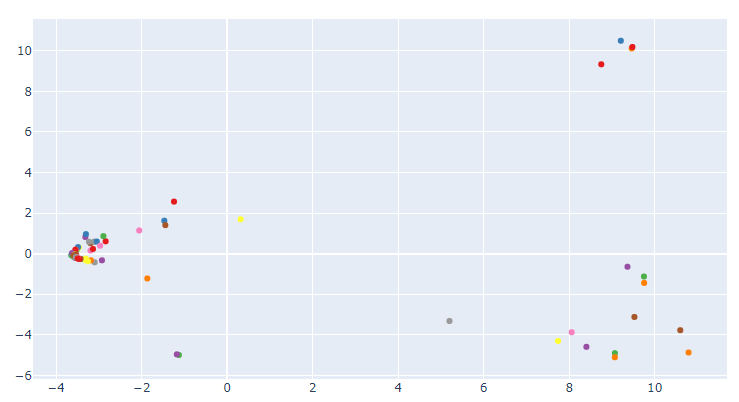
\includegraphics[width=\textwidth]{images/model_centrality_good2-8_2}
		\caption{Machine-1-4}
		\label{model-centrality-plot-good}
	\end{minipage}
	\begin{minipage}[b]{0.45\textwidth}
		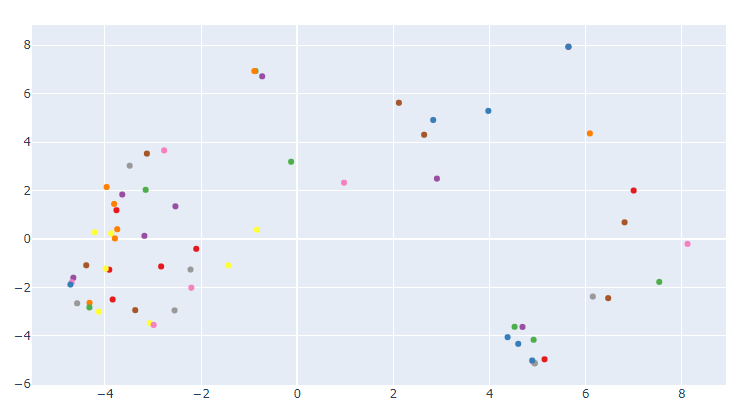
\includegraphics[width=\textwidth]{images/model_centrality_bad3-10_2}
		\caption{Machine-3-10}
		\label{model-centrality-plot-bad}
	\end{minipage}
\end{figure}

\begin{table}[]
	\caption{\label{mc-results}Risultati di correlazione per Model Centrality}
	\resizebox{\linewidth}{!}{%
		\begin{tabular}{|l||l|l|l|l||l|l|l|l||l|l|l|l|} 
			\hline
			Dataset           & \multicolumn{4}{c||}{SCORE CORRELATION} & \multicolumn{8}{c|}{RANK CORRELATION}                            \\ 
			\hline
			\multirow{2}{*}{} & \multicolumn{4}{c||}{PEARSON}           & \multicolumn{4}{c||}{KENDALL}  & \multicolumn{4}{c|}{SPEARMAN}   \\ 
			\cline{2-13}
			                & mv     & rr    & samp  & score  & mv    & rr    & samp  & score & mv    & rr           & samp   & score \\ 
			\hline
			2\_annthyroid   & 0.823  & 0.837 & 0.836 & 0.773  & 0.584 & 0.581 & 0.605 & 0.584 & 0.739 & 0.735        & 0.753  & 0.671 \\ 
			\hline
			6\_cardio       & 0.807  & 0.787 & 0.787 & 0.654  & 0.612 & 0.563 & 0.564 & 0.565 & 0.746 & 0.715        & 0.718  & 0.626 \\ 
			\hline
			11\_donors      & 0.514  & 0.529 & 0.526 & 0.423  & 0.541 & 0.511 & 0.529 & 0.475 & 0.665 & 0.650        & 0.670  & 0.559 \\ 
			\hline
			20\_letter      & 0.559  & 0.631 & 0.763 & 0.669  & 0.473 & 0.499 & 0.692 & 0.536 & 0.565 & 0.608        & 0.840  & 0.642 \\ 
			\hline
			23\_mammography & 0.795  & 0.829 & 0.801 & 0.607  & 0.694 & 0.722 & 0.649 & 0.439 & 0.834 & 0.821        & 0.809  & 0.561 \\ 
			\hline
			27\_PageBlocks  & 0.917  & 0.911 & 0.909 & 0.832  & 0.698 & 0.677 & 0.646 & 0.550 & 0.812 & 0.849        & 0.818  & 0.717 \\ 
			\hline
			31\_satimage-2  & 0.759  & 0.855 & 0.644 & 0.553  & 0.641 & 0.865 & 0.514 & 0.440 & 0.793 & 0.970        & 0.581  & 0.462 \\ 
			\hline
			32\_shuttle     & 0.489  & 0.846 & 0.827 & 0.661  & 0.446 & 0.774 & 0.770 & 0.565 & 0.456 & 0.894        & 0.890  & 0.728 \\ 
			\hline
			38\_thyroid     & 0.719  & 0.761 & 0.701 & 0.709  & 0.538 & 0.563 & 0.508 & 0.546 & 0.667 & 0.700        & 0.632  & 0.683 \\ 
			\hline
			40\_vowels      & 0.735  & 0.760 & 0.670 & 0.612  & 0.637 & 0.642 & 0.573 & 0.463 & 0.779 & 0.806        & 0.721  & 0.582 \\ 
			\hline
			41\_Waveform    & 0.428  & 0.464 & 0.440 & 0.481  & 0.466 & 0.582 & 0.569 & 0.423 & 0.572 & 0.709        & 0.647  & 0.541 \\ 
			\hline
			machine-1-1     & 0.561  & 0.582 & 0.641 & 0.556  & 0.458 & 0.458 & 0.499 & 0.468 & 0.558 & 0.572        & 0.607  & 0.595 \\ 
			\hline
			machine-1-2     & 0.842  & 0.877 & 0.866 & 0.771  & 0.633 & 0.732 & 0.723 & 0.570 & 0.834 & 0.839        & 0.836  & 0.738 \\ 
			\hline
			machine-1-3     & 0.949  & 0.836 & 0.828 & 0.480  & 0.855 & 0.633 & 0.645 & 0.437 & 0.934 & 0.841        & 0.826  & 0.428 \\ 
			\hline
			machine-1-4     & 0.966  & 0.949 & 0.917 & 0.576  & 0.835 & 0.706 & 0.711 & 0.412 & 0.927 & 0.842        & 0.840  & 0.553 \\ 
			\hline
			machine-1-5     & 0.441  & 0.494 & 0.465 & 0.353  & 0.458 & 0.477 & 0.456 & 0.432 & 0.587 & 0.514        & 0.584  & 0.419 \\ 
			\hline
			machine-1-6     & 0.588  & 0.551 & 0.576 & 0.585  & 0.550 & 0.527 & 0.528 & 0.521 & 0.621 & 0.582        & 0.578  & 0.601 \\ 
			\hline
			machine-1-7     & 0.630  & 0.596 & 0.626 & 0.597  & 0.546 & 0.491 & 0.543 & 0.467 & 0.693 & 0.636        & 0.680  & 0.593 \\ 
			\hline
			machine-1-8     & 0.594  & 0.563 & 0.553 & 0.628  & 0.494 & 0.421 & 0.492 & 0.406 & 0.590 & 0.433        & 0.514  & 0.553 \\ 
			\hline
			machine-2-1     & 0.791  & 0.838 & 0.847 & 0.566  & 0.561 & 0.595 & 0.563 & 0.465 & 0.653 & 0.687        & 0.690  & 0.535 \\ 
			\hline
			machine-2-2     & 0.822  & 0.824 & 0.827 & 0.683  & 0.608 & 0.594 & 0.565 & 0.503 & 0.794 & 0.770        & 0.739  & 0.601 \\ 
			\hline
			machine-2-3     & 0.825  & 0.827 & 0.834 & 0.606  & 0.648 & 0.610 & 0.638 & 0.444 & 0.819 & 0.771        & 0.798  & 0.546 \\ 
			\hline
			machine-2-4     & 0.307  & 0.309 & 0.285 & 0.192  & 0.357 & 0.348 & 0.301 & 0.389 & 0.411 & 0.369        & 0.310  & 0.317 \\ 
			\hline
			machine-2-5     & 0.044  & 0.133 & 0.126 & 0.136  & 0.332 & 0.379 & 0.351 & 0.383 & 0.380 & 0.356        & 0.326  & 0.325 \\ 
			\hline
			machine-2-6     & 0.896  & 0.872 & 0.893 & 0.568  & 0.703 & 0.648 & 0.679 & 0.511 & 0.816 & 0.823        & 0.801  & 0.594 \\ 
			\hline
			machine-2-7     & 0.882  & 0.885 & 0.839 & 0.820  & 0.683 & 0.718 & 0.662 & 0.648 & 0.823 & 0.848        & 0.806  & 0.806 \\ 
			\hline
			machine-2-8     & 0.991  & 0.989 & 0.983 & 0.803  & 0.861 & 0.876 & 0.847 & 0.532 & 0.961 & 0.966        & 0.950  & 0.627 \\ 
			\hline
			machine-2-9     & 0.627  & 0.649 & 0.664 & 0.420  & 0.492 & 0.472 & 0.480 & 0.414 & 0.597 & 0.569        & 0.571  & 0.409 \\ 
			\hline
			machine-3-1     & 0.458  & 0.467 & 0.532 & 0.485  & 0.431 & 0.444 & 0.453 & 0.381 & 0.483 & 0.504        & 0.591  & 0.427 \\ 
			\hline
			machine-3-2     & 0.613  & 0.646 & 0.670 & 0.727  & 0.595 & 0.595 & 0.627 & 0.638 & 0.753 & 0.761        & 0.785  & 0.814 \\ 
			\hline
			machine-3-3     & 0.345  & 0.379 & 0.365 & 0.388  & 0.420 & 0.384 & 0.364 & 0.468 & 0.475 & 0.451        & 0.434  & 0.454 \\ 
			\hline
			machine-3-4     & 0.158  & 0.168 & 0.224 & -0.036 & 0.271 & 0.241 & 0.293 & 0.095 & 0.331 & 0.281        & 0.334  & 0.154 \\ 
			\hline
			machine-3-5     & 0.857  & 0.871 & 0.864 & 0.521  & 0.699 & 0.774 & 0.759 & 0.470 & 0.817 & 0.880        & 0.870  & 0.523 \\ 
			\hline
			machine-3-6     & 0.338  & 0.311 & 0.292 & 0.069  & 0.393 & 0.305 & 0.391 & 0.365 & 0.463 & 0.379        & 0.351  & 0.312 \\ 
			\hline
			machine-3-7     & 0.308  & 0.361 & 0.321 & 0.299  & 0.469 & 0.447 & 0.452 & 0.365 & 0.493 & 0.464        & 0.474  & 0.443 \\ 
			\hline
			machine-3-8     & 0.648  & 0.651 & 0.700 & 0.471  & 0.579 & 0.547 & 0.590 & 0.412 & 0.696 & 0.682        & 0.727  & 0.570 \\ 
			\hline
			machine-3-9     & 0.580  & 0.477 & 0.496 & 0.431  & 0.665 & 0.589 & 0.588 & 0.463 & 0.833 & 0.710        & 0.719  & 0.595 \\ 
			\hline
			machine-3-10    & -0.009 & 0.015 & 0.116 & 0.010  & 0.269 & 0.288 & 0.300 & 0.210 & 0.348 & 0.322        & 0.324  & 0.272 \\ 
			\hline
			machine-3-11    & 0.837  & 0.626 & 0.560 & 0.372  & 0.640 & 0.465 & 0.332 & 0.348 & 0.813 & 0.470        & 0.401  & 0.315 \\ 
			\hline
			AVG             & 0.627  & 0.640 & 0.636 & 0.514  & 0.560 & 0.558 & 0.550 & 0.457 & 0.670 & 0.661        & 0.655  & 0.536 \\ 
			\hline
			STD             & 0.25   & 0.24  & 0.229 & 0.214  & 0.142 & 0.149 & 0.135 & 0.102 & 0.169 & 0.186        & 0.177  & 0.146 \\
			\hline
		\end{tabular}
	}
\end{table}

\newpage
\subsubsection{Performance on Injected Synthetic Anomalies}
Passando alla metrica surrogata usante le pseudo-etichette dopo l'iniezione di anomalie, le tipologie di anomalia iniettate sono Spike, Scale, Growing e Mix dove Mix rappresentano i dataset a cui sono stati iniettate tutte e 3 le tipologie di anomalie trattate a inizio capitolo. Possiamo notare in tabella \ref{pai-results} come generalmente le performance siano inferiori rispetto alla tecnica del Model Centrality. I motivi di ciò possono ricondursi agli aspetti negativi introdotti precedentemente che riguardano questo approccio: 
\begin{enumerate}
	\item come le anomalie vengono generate
	\item le anomalie reali vengano ignorate
\end{enumerate}
Il primo punto non é banale, avere una conoscenza forte dal dataset di riferimento permette di creare anomalie che possano risultare realistiche ma spesso la ciò non é possibile. Attraverso metodi statistici si possono estrarre informazioni riguardanti l'andamento e l'evoluzione dei dati ma spesso le anomalie non seguono un pattern preciso rendendo quindi la generazione di queste un problema non triviale. 
Vediamo ora alcuni esempi di come le performance variano in base al dataset ed al tipo di anomalia iniettata. Le performance dell'anomia Spike sul dataset Shuttle sono buone e a conferma di ciò si puo vedere in figura \ref{shuttle-inj} come le anomalie prevalenti siano proprio di tipo Spike.
Al contrario, Machine-3-5 ha performance basse per quanto riguarda Growing, Spike e Mix, ma ottiene un punteggio di 0.84 su Scale. La figura \ref{machine-3-5-inj} mostra come i punti anomali abbiano intervalli con valori scalati verso l'alto. Infine, Machine-28 é quello con le performance Mix più alte, a riprova del fatto che nell'immagine \ref{machine-2-8-inj} si possono notare sia spike, sia intervalli anomali e sia valori crescenti nel tempo.
Il secondo punto trattato può impattare negativamente i risultati in quanto é possibile che il modello vada a etichettare le anomalie reali come positive, nonostante abbiano delle etichette pseudo-negative. Una soluzione a questo problema potrebbe essere quello di ricercare una finestra temporale del dataset che sia il più pulita possibile dalla anomalie per poi andare ad effettuare le iniezioni di anomalia.
Anche in questo caso ci troviamo di fronte a tre metodi con performance simili con un quarto, in questo caso Growing, generalmente meno performante.
\begin{figure}[htp]% [H] is so declass\'e!
	\centering
	\begin{minipage}{0.5\textwidth}
		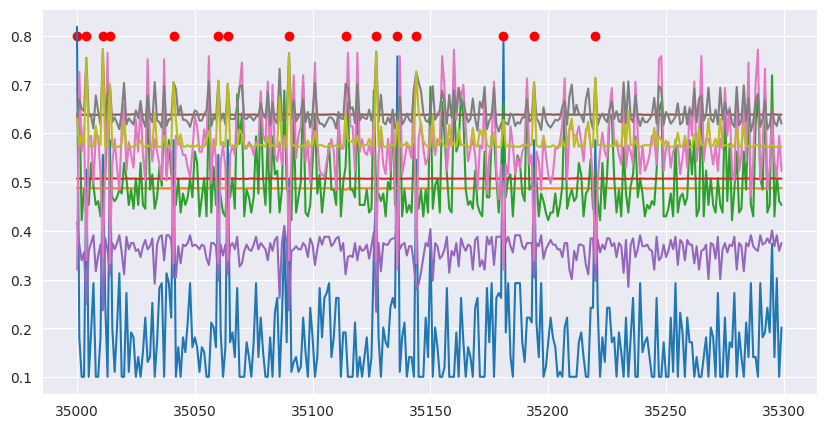
\includegraphics[width=\textwidth]{images/shuttle_good_inj_spike.png}
		\caption{Shuttle}
		\label{shuttle-inj}
	\end{minipage}\hfill
	\begin{minipage}{0.5\textwidth}
		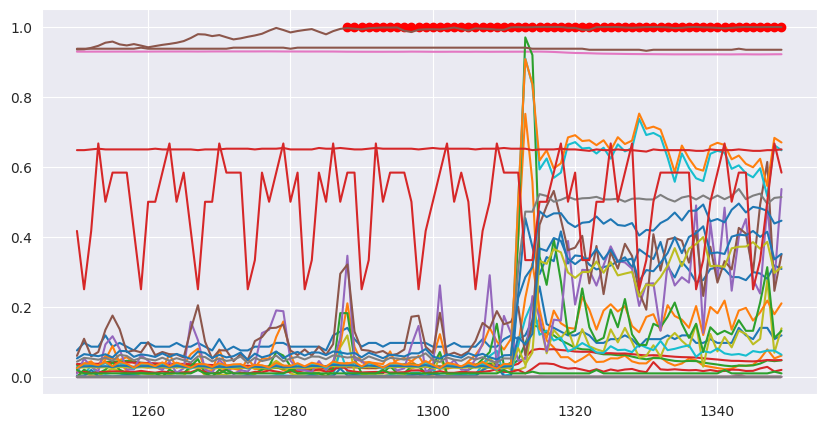
\includegraphics[width=\textwidth]{images/machine-3-5_bad_inj_good_scale.png}
		\caption{Machine-3-5}
		\label{machine-3-5-inj}
	\end{minipage}\par
	\vskip\floatsep% normal separation between figures
	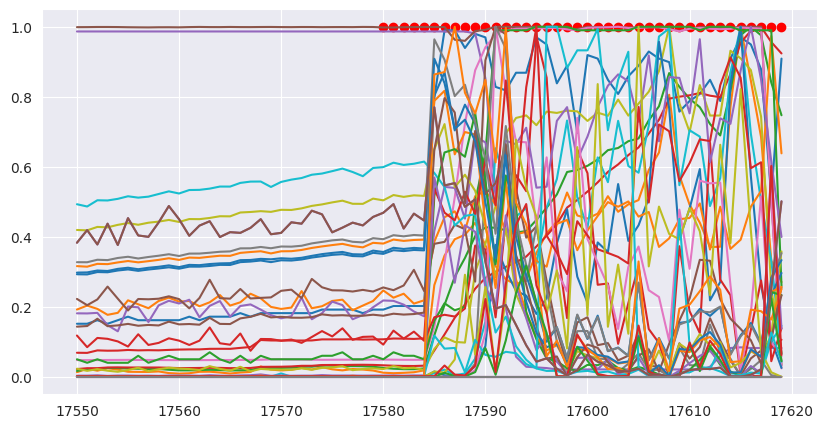
\includegraphics[width=0.5\textwidth]{images/machine-2-8_good_inj_mix.png}
	\caption{Machine-2-8}
	\label{machine-2-8-inj}
\end{figure}

\begin{table}[]
	\caption{\label{pai-results}Risultati di correlazione per Performance on Injected Synthetic Anomalies}
	\resizebox{\linewidth}{!}{%
		\begin{tabular}{|l||l|l|l|l||l|l|l|l||l|l|l|l|} 
			\hline
			Dataset           & \multicolumn{4}{c||}{SCORE CORRELATION} & \multicolumn{8}{c|}{RANK CORRELATION}                            \\ 
			\hline
			\multirow{2}{*}{} & \multicolumn{4}{c||}{PEARSON}           & \multicolumn{4}{c||}{KENDALL}  & \multicolumn{4}{c|}{SPEARMAN}   \\ 
			\cline{2-13}
			                & wander & spike & scale & mix   & wander & spike & scale & mix   & wander & spike        & scale & mix   \\ 
			\hline
			2\_annthyroid   & 0.111  & 0.272 & 0.331 & 0.196 & 0.267  & 0.440 & 0.465 & 0.408 & 0.281  & 0.487        & 0.414 & 0.457 \\ 
			\hline
			6\_cardio       & 0.269  & 0.575 & 0.554 & 0.381 & 0.129  & 0.337 & 0.431 & 0.356 & 0.176  & 0.406        & 0.416 & 0.396 \\ 
			\hline
			11\_donors      & 0.331  & 0.391 & 0.316 & 0.303 & 0.472  & 0.422 & 0.442 & 0.443 & 0.491  & 0.550        & 0.575 & 0.573 \\ 
			\hline
			20\_letter      & 0.457  & 0.577 & 0.811 & 0.560 & 0.489  & 0.607 & 0.718 & 0.527 & 0.563  & 0.742        & 0.805 & 0.597 \\ 
			\hline
			23\_mammography & 0.378  & 0.401 & 0.396 & 0.494 & 0.423  & 0.562 & 0.486 & 0.535 & 0.530  & 0.671        & 0.591 & 0.597 \\ 
			\hline
			27\_PageBlocks  & 0.357  & 0.340 & 0.430 & 0.368 & 0.384  & 0.374 & 0.451 & 0.365 & 0.473  & 0.477        & 0.469 & 0.461 \\ 
			\hline
			31\_satimage-2  & 0.092  & 0.090 & 0.110 & 0.231 & 0.310  & 0.228 & 0.304 & 0.309 & 0.393  & 0.330        & 0.314 & 0.303 \\ 
			\hline
			32\_shuttle     & 0.308  & 0.333 & 0.330 & 0.355 & 0.319  & 0.303 & 0.360 & 0.344 & 0.408  & 0.368        & 0.436 & 0.414 \\ 
			\hline
			38\_thyroid     & 0.093  & 0.164 & 0.159 & 0.117 & 0.362  & 0.390 & 0.474 & 0.362 & 0.398  & 0.354        & 0.459 & 0.384 \\ 
			\hline
			40\_vowels      & 0.470  & 0.667 & 0.581 & 0.712 & 0.429  & 0.611 & 0.564 & 0.607 & 0.527  & 0.761        & 0.623 & 0.759 \\ 
			\hline
			41\_Waveform    & 0.810  & 0.775 & 0.679 & 0.764 & 0.627  & 0.571 & 0.580 & 0.639 & 0.783  & 0.737        & 0.721 & 0.823 \\ 
			\hline
			machine-1-1     & 0.379  & 0.490 & 0.597 & 0.583 & 0.425  & 0.407 & 0.697 & 0.535 & 0.557  & 0.584        & 0.835 & 0.634 \\ 
			\hline
			machine-1-2     & 0.339  & 0.373 & 0.393 & 0.364 & 0.399  & 0.316 & 0.345 & 0.351 & 0.457  & 0.354        & 0.417 & 0.368 \\ 
			\hline
			machine-1-3     & 0.117  & 0.487 & 0.335 & 0.368 & 0.334  & 0.561 & 0.325 & 0.469 & 0.210  & 0.682        & 0.180 & 0.566 \\ 
			\hline
			machine-1-4     & 0.170  & 0.206 & 0.347 & 0.193 & 0.354  & 0.444 & 0.131 & 0.309 & 0.229  & 0.489        & 0.238 & 0.313 \\ 
			\hline
			machine-1-5     & 0.108  & 0.468 & 0.209 & 0.417 & 0.316  & 0.468 & 0.383 & 0.473 & 0.360  & 0.545        & 0.325 & 0.415 \\ 
			\hline
			machine-1-6     & 0.423  & 0.566 & 0.471 & 0.441 & 0.351  & 0.449 & 0.473 & 0.405 & 0.470  & 0.575        & 0.562 & 0.494 \\ 
			\hline
			machine-1-7     & 0.301  & 0.436 & 0.351 & 0.318 & 0.329  & 0.541 & 0.432 & 0.389 & 0.397  & 0.615        & 0.440 & 0.328 \\ 
			\hline
			machine-1-8     & 0.342  & 0.472 & 0.538 & 0.357 & 0.426  & 0.429 & 0.478 & 0.368 & 0.454  & 0.447        & 0.596 & 0.350 \\ 
			\hline
			machine-2-1     & 0.516  & 0.547 & 0.497 & 0.469 & 0.502  & 0.515 & 0.479 & 0.397 & 0.576  & 0.560        & 0.446 & 0.410 \\ 
			\hline
			machine-2-2     & 0.500  & 0.464 & 0.462 & 0.516 & 0.459  & 0.403 & 0.455 & 0.476 & 0.588  & 0.523        & 0.554 & 0.591 \\ 
			\hline
			machine-2-3     & 0.555  & 0.471 & 0.470 & 0.550 & 0.540  & 0.479 & 0.428 & 0.567 & 0.647  & 0.556        & 0.540 & 0.714 \\ 
			\hline
			machine-2-4     & 0.201  & 0.422 & 0.540 & 0.522 & 0.243  & 0.425 & 0.439 & 0.517 & 0.291  & 0.443        & 0.582 & 0.584 \\ 
			\hline
			machine-2-5     & 0.459  & 0.463 & 0.401 & 0.451 & 0.498  & 0.545 & 0.558 & 0.638 & 0.579  & 0.632        & 0.712 & 0.781 \\ 
			\hline
			machine-2-6     & 0.156  & 0.438 & 0.132 & 0.404 & 0.222  & 0.462 & 0.270 & 0.492 & 0.228  & 0.569        & 0.267 & 0.596 \\ 
			\hline
			machine-2-7     & 0.391  & 0.343 & 0.450 & 0.360 & 0.476  & 0.433 & 0.468 & 0.307 & 0.495  & 0.414        & 0.560 & 0.382 \\ 
			\hline
			machine-2-8     & 0.776  & 0.330 & 0.042 & 0.771 & 0.500  & 0.345 & 0.094 & 0.510 & 0.598  & 0.423        & 0.052 & 0.575 \\ 
			\hline
			machine-2-9     & 0.463  & 0.361 & 0.329 & 0.322 & 0.512  & 0.464 & 0.366 & 0.404 & 0.577  & 0.574        & 0.429 & 0.491 \\ 
			\hline
			machine-3-1     & 0.348  & 0.366 & 0.721 & 0.411 & 0.571  & 0.507 & 0.667 & 0.520 & 0.614  & 0.566        & 0.813 & 0.580 \\ 
			\hline
			machine-3-2     & 0.443  & 0.401 & 0.374 & 0.318 & 0.474  & 0.493 & 0.402 & 0.356 & 0.453  & 0.483        & 0.455 & 0.397 \\ 
			\hline
			machine-3-3     & 0.458  & 0.336 & 0.404 & 0.347 & 0.508  & 0.336 & 0.547 & 0.467 & 0.557  & 0.432        & 0.619 & 0.457 \\ 
			\hline
			machine-3-4     & 0.351  & 0.363 & 0.408 & 0.360 & 0.442  & 0.378 & 0.415 & 0.409 & 0.445  & 0.477        & 0.542 & 0.520 \\ 
			\hline
			machine-3-5     & 0.077  & 0.188 & 0.841 & 0.036 & 0.117  & 0.255 & 0.771 & 0.035 & 0.121  & 0.240        & 0.823 & 0.056 \\ 
			\hline
			machine-3-6     & 0.513  & 0.445 & 0.359 & 0.516 & 0.450  & 0.421 & 0.338 & 0.460 & 0.576  & 0.537        & 0.314 & 0.462 \\ 
			\hline
			machine-3-7     & 0.470  & 0.486 & 0.484 & 0.406 & 0.487  & 0.551 & 0.398 & 0.493 & 0.592  & 0.702        & 0.499 & 0.484 \\ 
			\hline
			machine-3-8     & 0.371  & 0.355 & 0.202 & 0.357 & 0.464  & 0.484 & 0.271 & 0.439 & 0.432  & 0.588        & 0.350 & 0.540 \\ 
			\hline
			machine-3-9     & 0.339  & 0.310 & 0.447 & 0.378 & 0.382  & 0.387 & 0.591 & 0.472 & 0.383  & 0.484        & 0.658 & 0.463 \\ 
			\hline
			machine-3-10    & 0.344  & 0.465 & 0.398 & 0.379 & 0.428  & 0.530 & 0.541 & 0.516 & 0.486  & 0.623        & 0.613 & 0.555 \\ 
			\hline
			machine-3-11    & 0.516  & 0.663 & 0.394 & 0.693 & 0.496  & 0.504 & 0.395 & 0.551 & 0.503  & 0.607        & 0.461 & 0.693 \\ 
			\hline
			AVG             & 0.362  & 0.418 & 0.418 & 0.413 & 0.408  & 0.446 & 0.447 & 0.442 & 0.459  & 0.528        & 0.505 & 0.502 \\ 
			\hline
			STD             & 0.169  & 0.136 & 0.172 & 0.157 & 0.11   & 0.092 & 0.139 & 0.11  & 0.141  & 0.119        & 0.176 & 0.147 \\
			\hline
		\end{tabular}
	}
\end{table}

\newpage
\subsubsection{Clustering Cohesion}
Questa metrica surrogata invece va a favorire soluzioni cui le anomalie sono ben separate dai dati normali, infatti le performance variano di molto per ogni dataset preso in considerazione con un AVG score più basso rispetto alle altre due metriche (tabella \ref{cc-results}).


\begin{table}[]
	\caption{\label{cc-results}Risultati di correlazione per Clustering Cohesion}
	\resizebox{\columnwidth}{!}{%
		\begin{tabular}{|l|l|l|l|}
			\hline
			Dataset         & \multicolumn{1}{c|}{SCORE CORRELATION} & \multicolumn{2}{c|}{RANK CORRELATION}                         \\  \hline
			                & \multicolumn{1}{c|}{PEARSON} & \multicolumn{1}{c|}{KENDALL} & \multicolumn{1}{c|}{SPEARMAN} \\ \hline
			2\_annthyroid   & 0.821                        & 0.432                        & 0.557                         \\ \hline
			6\_cardio       & 0.409                        & 0.375                        & 0.436                         \\ \hline
			11\_donors      & 0.096                        & 0.111                        & -0.049                        \\ \hline
			20\_letter      & -0.034                       & 0.061                        & -0.049                        \\ \hline
			23\_mammography & 0.368                        & 0.369                        & 0.469                         \\ \hline
			27\_PageBlocks  & 0.837                        & 0.496                        & 0.487                         \\ \hline
			31\_satimage-2  & 0.467                        & 0.389                        & 0.355                         \\ \hline
			32\_shuttle     & 0.830                        & 0.706                        & 0.832                         \\ \hline
			38\_thyroid     & 0.606                        & 0.483                        & 0.581                         \\ \hline
			40\_vowels      & 0.444                        & 0.393                        & 0.487                         \\ \hline
			41\_Waveform    & 0.109                        & 0.232                        & 0.215                         \\ \hline
			machine-1-1     & -0.103                       & 0.100                        & -0.055                        \\ \hline
			machine-1-2     & 0.517                        & 0.421                        & 0.540                         \\ \hline
			machine-1-3     & -0.166                       & -0.010                       & -0.137                        \\ \hline
			machine-1-4     & -0.109                       & 0.045                        & -0.033                        \\ \hline
			machine-1-5     & 0.376                        & 0.435                        & 0.438                         \\ \hline
			machine-1-6     & -0.332                       & -0.215                       & -0.404                        \\ \hline
			machine-1-7     & 0.041                        & -0.066                       & -0.189                        \\ \hline
			machine-1-8     & 0.004                        & 0.107                        & -0.030                        \\ \hline
			machine-2-1     & -0.043                       & 0.112                        & 0.032                         \\ \hline
			machine-2-2     & 0.474                        & 0.386                        & 0.357                         \\ \hline
			machine-2-3     & 0.786                        & 0.505                        & 0.636                         \\ \hline
			machine-2-4     & 0.343                        & 0.193                        & 0.167                         \\ \hline
			machine-2-5     & -0.092                       & -0.111                       & -0.267                        \\ \hline
			machine-2-6     & 0.446                        & 0.315                        & 0.308                         \\ \hline
			machine-2-7     & 0.621                        & 0.483                        & 0.574                         \\ \hline
			machine-2-8     & 0.658                        & 0.493                        & 0.573                         \\ \hline
			machine-2-9     & 0.309                        & 0.324                        & 0.357                         \\ \hline
			machine-3-1     & 0.395                        & 0.305                        & 0.289                         \\ \hline
			machine-3-2     & 0.468                        & 0.442                        & 0.445                         \\ \hline
			machine-3-3     & -0.335                       & -0.155                       & -0.343                        \\ \hline
			machine-3-4     & -0.016                       & 0.117                        & 0.028                         \\ \hline
			machine-3-5     & 0.682                        & 0.514                        & 0.607                         \\ \hline
			machine-3-6     & 0.093                        & -0.009                       & -0.112                        \\ \hline
			machine-3-7     & 0.258                        & 0.371                        & 0.324                         \\ \hline
			machine-3-8     & 0.204                        & 0.145                        & 0.128                         \\ \hline
			machine-3-9     & 0.299                        & 0.170                        & 0.119                         \\ \hline
			machine-3-10    & -0.207                       & -0.003                       & -0.182                        \\ \hline
			machine-3-11    & -0.050                       & 0.095                        & -0.006                        \\ \hline
			AVG             & 0.269                        & 0.245                        & 0.217                         \\ \hline
			STD             & 0.329                        & 0.218                        & 0.309                         \\ \hline
		\end{tabular}%
	}
\end{table}

Alcuni dataset, come annthyroid, page blocks, shuttle e waveform hanno una distribuzione dei dati tale da essere facilmente clusterizzabile da metodi come DBSCAN, usato appunto in questa metrica surrogata. Questo permette quindi di favorire quei modelli che riescono a trovare questa separazione tra i punti normali ed i punti anomali.
Gli altri dataset invece faticano a trovare una forte correlazione con il ranking supervisionato, proprio per il fatto che in questo caso i punti anomali sono altamente "mischiati" in mezzo a quelli normali.
Questa tecnica e quindi consigliabile se si hanno conoscenze pregresse sul dataset che si vuole analizzare e si nota una chiara separazione dei dati. Un esempio sono due dataset, Machine-2-3 e Machine-1-7 in cui il primo ha una correlazione di Clustering Cohesion con il ranking supervisionato discretamente buona. A dimostrare questo si può notare come nella prima figura i dati siano tutti concentrati nella zona di destra ed inoltre quella zona é coperta principalmente da punti normali dove invece i punti anomali sono sparsi nel resto del piano. 
Al contrario il dataset Machine-1-7 ha una correlazione nulla e graficamente il plot mostra come la distribuzione dei punti sia più omogenea e le anomalie non sono ben separate come nel caso precedente. 
\begin{center}
	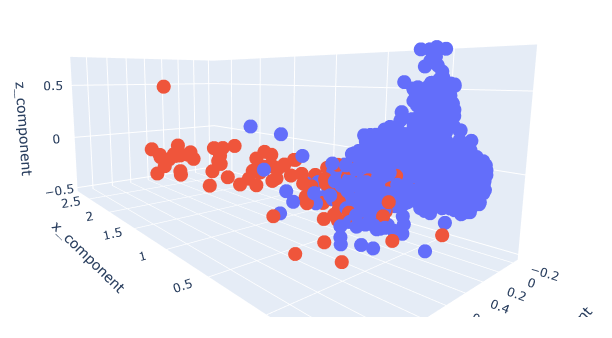
\includegraphics[width=9cm, scale=1]{images/scatter_cluster_good}
    \captionsetup{type=figure}
	\captionof{figure}{Scatter Plot Machine-2-3}
\end{center}
\begin{center}
	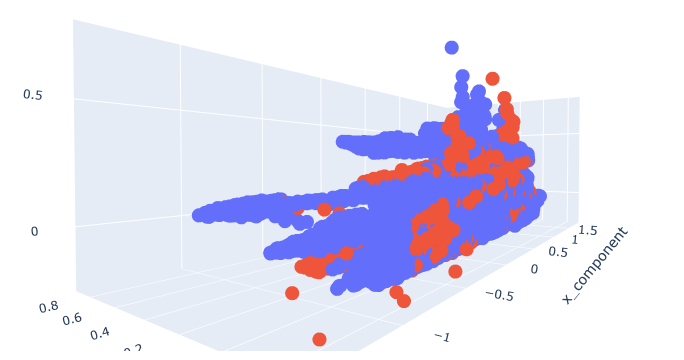
\includegraphics[width=9cm, scale=1]{images/scatter_cluster}
    \captionsetup{type=figure}
	\captionof{figure}{Scatter Plot Machine-1-7}
\end{center}

\newpage
\subsubsection{Rank Aggregation}
A questo punto ci si può concentrare sulle varie tecniche di aggregazione. L'aggregazione è stata fatta andando a considerare sempre tutte e 3 le metriche surrogate, senza fare eccezione nonostante ci fossero dataset in cui alcune metriche surrogate avevano performance particolarmente basse. 
Si può vedere, in tabella \ref{agg-results}, come il metodo ottimale di aggregazione, che ricordiamo essere NP-Hard, produca i risultati migliori. 
I valori medi rispetto ai dataset si aggirano intorno al range [0.4,0.6], in linea con le performance di Model Centrality e migliori rispetto a Performance on Injected Synthetic Anomalies e Clustering Cohesion. Questo vuol dire che i metodi di aggregazione riescono comunque a produrre buoni risultati nonostante le metriche surrogante non funzioni sempre bene. 
Questo tipo di aggregazione permette di avere risultati migliori quando non si ha la certezza che una sola metrica surrogata sia sufficiente. Potrebbe comunque essere utile un'analisi specifica per andare a prendere in considerazione soltanto quelle metriche surrogate, o più nello specifico i metodi utilizzati al loro interno (Round Robin, Majority Vote, Sampling o Scale, Spike, Growing, Mix), che potrebbero funzionare meglio per uno specifico dataset. 


\begin{table}[]
	\caption{\label{agg-results}Risultati di correlazione per aggregazione}
	\resizebox{\linewidth}{!}{%
		\begin{tabular}{|l||l|l|l|l||l|l|l|l||l|l|l|l|} 
			\hline
			Dataset           & \multicolumn{4}{c||}{SCORE CORRELATION} & \multicolumn{8}{c|}{RANK CORRELATION}                            \\ 
			\hline
			\multirow{2}{*}{} & \multicolumn{4}{c||}{PEARSON}           & \multicolumn{4}{c||}{KENDALL}  & \multicolumn{4}{c|}{SPEARMAN}   \\ 
			\cline{2-13}
			                & score & borda & rborda & opt   & score & borda & rborda & opt   & score & borda        & rborda & opt   \\ 
			\hline
			2\_annthyroid   & 0.795 & 0.644 & 0.394  & 0.768 & 0.486 & 0.499 & 0.382  & 0.586 & 0.550 & 0.587        & 0.331 & 0.696 \\ 
			\hline
			6\_cardio       & 0.758 & 0.589 & 0.409  & 0.597 & 0.578 & 0.416 & 0.374  & 0.550 & 0.693 & 0.545        & 0.447 & 0.572 \\ 
			\hline
			11\_donors      & 0.404 & 0.633 & 0.164  & 0.541 & 0.348 & 0.553 & 0.129  & 0.573 & 0.430 & 0.672        & 0.195 & 0.683 \\ 
			\hline
			20\_letter      & 0.595 & 0.561 & 0.436  & 0.664 & 0.493 & 0.423 & 0.418  & 0.546 & 0.606 & 0.557        & 0.406 & 0.639 \\ 
			\hline
			23\_mammography & 0.681 & 0.770 & 0.489  & 0.793 & 0.495 & 0.587 & 0.427  & 0.654 & 0.599 & 0.748        & 0.427 & 0.822 \\ 
			\hline
			27\_PageBlocks  & 0.843 & 0.753 & 0.395  & 0.860 & 0.594 & 0.551 & 0.323  & 0.659 & 0.690 & 0.713        & 0.375 & 0.822 \\ 
			\hline
			31\_satimage-2  & 0.574 & 0.761 & 0.489  & 0.730 & 0.428 & 0.559 & 0.389  & 0.630 & 0.584 & 0.736        & 0.457 & 0.816 \\ 
			\hline
			32\_shuttle     & 0.562 & 0.843 & 0.696  & 0.899 & 0.500 & 0.644 & 0.592  & 0.755 & 0.590 & 0.806        & 0.674 & 0.882 \\ 
			\hline
			38\_thyroid     & 0.623 & 0.616 & 0.367  & 0.644 & 0.477 & 0.451 & 0.390  & 0.526 & 0.536 & 0.561        & 0.334 & 0.655 \\ 
			\hline
			40\_vowels      & 0.765 & 0.813 & 0.578  & 0.807 & 0.649 & 0.632 & 0.430  & 0.661 & 0.833 & 0.816        & 0.546 & 0.858 \\ 
			\hline
			41\_Waveform    & 0.581 & 0.623 & 0.536  & 0.521 & 0.560 & 0.464 & 0.435  & 0.576 & 0.673 & 0.586        & 0.540 & 0.668 \\ 
			\hline
			machine-1-1     & 0.464 & 0.556 & 0.311  & 0.620 & 0.486 & 0.434 & 0.292  & 0.564 & 0.526 & 0.581        & 0.302 & 0.684 \\ 
			\hline
			machine-1-2     & 0.820 & 0.797 & 0.423  & 0.777 & 0.623 & 0.591 & 0.423  & 0.632 & 0.841 & 0.753        & 0.413 & 0.782 \\ 
			\hline
			machine-1-3     & 0.245 & 0.686 & 0.416  & 0.623 & 0.294 & 0.596 & 0.437  & 0.561 & 0.291 & 0.689        & 0.413 & 0.651 \\ 
			\hline
			machine-1-4     & 0.411 & 0.577 & 0.390  & 0.475 & 0.390 & 0.491 & 0.397  & 0.496 & 0.470 & 0.589        & 0.449 & 0.512 \\ 
			\hline
			machine-1-5     & 0.496 & 0.581 & 0.423  & 0.477 & 0.429 & 0.411 & 0.480  & 0.460 & 0.567 & 0.537        & 0.448 & 0.589 \\ 
			\hline
			machine-1-6     & 0.476 & 0.302 & 0.259  & 0.554 & 0.376 & 0.342 & 0.292  & 0.361 & 0.363 & 0.381        & 0.291 & 0.437 \\ 
			\hline
			machine-1-7     & 0.413 & 0.354 & 0.250  & 0.375 & 0.372 & 0.314 & 0.312  & 0.378 & 0.500 & 0.410        & 0.322 & 0.451 \\ 
			\hline
			machine-1-8     & 0.385 & 0.417 & 0.243  & 0.507 & 0.319 & 0.347 & 0.254  & 0.406 & 0.392 & 0.311        & 0.227 & 0.511 \\ 
			\hline
			machine-2-1     & 0.606 & 0.510 & 0.396  & 0.559 & 0.427 & 0.436 & 0.395  & 0.497 & 0.554 & 0.446        & 0.350 & 0.513 \\ 
			\hline
			machine-2-2     & 0.761 & 0.658 & 0.426  & 0.623 & 0.434 & 0.492 & 0.434  & 0.478 & 0.560 & 0.577        & 0.418 & 0.607 \\ 
			\hline
			machine-2-3     & 0.861 & 0.876 & 0.825  & 0.895 & 0.709 & 0.783 & 0.632  & 0.760 & 0.816 & 0.881        & 0.805 & 0.886 \\ 
			\hline
			machine-2-4     & 0.453 & 0.497 & 0.432  & 0.511 & 0.451 & 0.431 & 0.489  & 0.496 & 0.541 & 0.513        & 0.473 & 0.572 \\ 
			\hline
			machine-2-5     & 0.129 & 0.425 & 0.320  & 0.297 & 0.241 & 0.396 & 0.363  & 0.399 & 0.294 & 0.346        & 0.378 & 0.469 \\ 
			\hline
			machine-2-6     & 0.725 & 0.726 & 0.312  & 0.789 & 0.498 & 0.531 & 0.314  & 0.584 & 0.634 & 0.676        & 0.335 & 0.738 \\ 
			\hline
			machine-2-7     & 0.792 & 0.776 & 0.554  & 0.839 & 0.591 & 0.576 & 0.457  & 0.626 & 0.730 & 0.717        & 0.600 & 0.762 \\ 
			\hline
			machine-2-8     & 0.933 & 0.839 & 0.575  & 0.903 & 0.774 & 0.726 & 0.505  & 0.763 & 0.870 & 0.825        & 0.566 & 0.882 \\ 
			\hline
			machine-2-9     & 0.587 & 0.624 & 0.532  & 0.629 & 0.535 & 0.444 & 0.484  & 0.549 & 0.623 & 0.584        & 0.480 & 0.580 \\ 
			\hline
			machine-3-1     & 0.554 & 0.624 & 0.451  & 0.670 & 0.482 & 0.486 & 0.398  & 0.578 & 0.565 & 0.574        & 0.454 & 0.661 \\ 
			\hline
			machine-3-2     & 0.661 & 0.687 & 0.497  & 0.683 & 0.608 & 0.573 & 0.478  & 0.607 & 0.779 & 0.656        & 0.566 & 0.676 \\ 
			\hline
			machine-3-3     & 0.065 & 0.287 & 0.256  & 0.341 & 0.112 & 0.242 & 0.325  & 0.356 & 0.154 & 0.261        & 0.329 & 0.415 \\ 
			\hline
			machine-3-4     & 0.239 & 0.387 & 0.394  & 0.203 & 0.392 & 0.332 & 0.325  & 0.428 & 0.351 & 0.373        & 0.374 & 0.395 \\ 
			\hline
			machine-3-5     & 0.844 & 0.622 & 0.454  & 0.675 & 0.744 & 0.503 & 0.463  & 0.569 & 0.866 & 0.582        & 0.437 & 0.648 \\ 
			\hline
			machine-3-6     & 0.363 & 0.390 & 0.294  & 0.401 & 0.318 & 0.385 & 0.270  & 0.437 & 0.305 & 0.300        & 0.260 & 0.523 \\ 
			\hline
			machine-3-7     & 0.355 & 0.496 & 0.497  & 0.424 & 0.425 & 0.418 & 0.436  & 0.520 & 0.485 & 0.419        & 0.404 & 0.536 \\ 
			\hline
			machine-3-8     & 0.586 & 0.660 & 0.534  & 0.630 & 0.468 & 0.500 & 0.427  & 0.552 & 0.589 & 0.597        & 0.535 & 0.642 \\ 
			\hline
			machine-3-9     & 0.496 & 0.677 & 0.526  & 0.590 & 0.496 & 0.529 & 0.448  & 0.604 & 0.555 & 0.622        & 0.526 & 0.701 \\ 
			\hline
			machine-3-10    & 0.021 & 0.365 & 0.382  & 0.262 & 0.152 & 0.259 & 0.379  & 0.313 & 0.175 & 0.327        & 0.343 & 0.395 \\ 
			\hline
			machine-3-11    & 0.590 & 0.612 & 0.553  & 0.639 & 0.467 & 0.449 & 0.426  & 0.511 & 0.469 & 0.596        & 0.558 & 0.642 \\ 
			\hline
			AVG             & 0.552 & 0.605 & 0.433  & 0.610 & 0.467 & 0.482 & 0.401  & 0.544 & 0.555 & 0.576        & 0.430 & 0.640 \\ 
			\hline
			STD             & 0.22  & 0.154 & 0.127  & 0.177 & 0.141 & 0.115 & 0.09   & 0.107 & 0.177 & 0.156        & 0.121 & 0.138 \\
			\hline
		\end{tabular}
	}
\end{table}

\newpage
\subsubsection{Variazione di K}
Interessante vedere come Robust Borda, che sulla carta dovrebbe avere performance migliori, sia in verità inferiore alla sua versione standard Borda. Un motivo di ciò può risiedere nel fatto che ci sono modelli che sono nelle posizioni più alte per quanto riguarda alcune metriche surrogate ma che performano sufficientemente male in altre e vengono quindi penalizzate troppo.
Si può vedere infatti, nell'immagine \ref{varying-k}, che all'aumentare del fattore K aumentano le performance di Robust Borda, fino arrivare al valore massimo con K=N, ovvero Borda normale.
Il metodo di AVG Score é il più semplice ma produce anche risultati più scarsi. Nel nostro caso, con sole 3 metriche surrogate che vengono aggregate, l'utilizzo del metodo ottimale risulta la scelta migliore nonostante la complessità temporale sia più alta. Se si fossero prese in considerazione più metriche, questo approccio non sarebbe più possibile proprio per la natura NP-Hard del problema.

\begin{figure}[t]
	\centering
	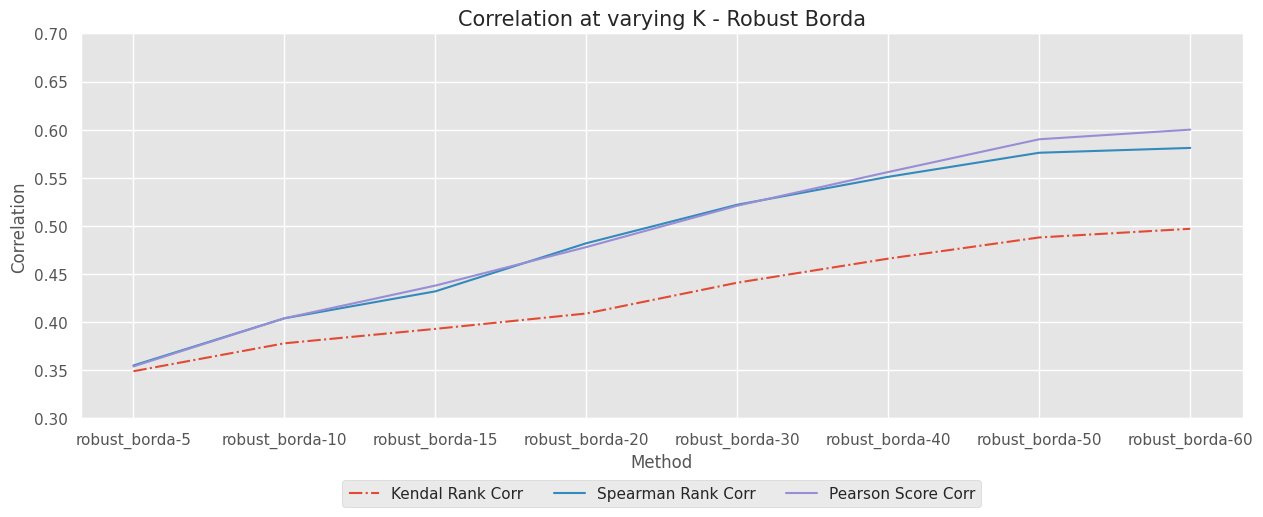
\includegraphics[width=14cm, scale=1]{images/varying-k}
	\caption{Performance di Robust Borda al variare del parametro K}
	\label{varying-k}
		
\end{figure}

\subsubsection{Ripetitività}
Alcune metriche surrogate includono al loro interno un fattore di casualità, in particolare Sampling e tutte e 4 le tecniche di Anomaly Injection. Il primo metodo può variare ad ogni suo utilizzo in quanto per ogni sample viene scelto a caso quale modello usare come riferimento per l'etichetta. Invece i metodi di Anomaly Injection genereranno sempre anomalie differenti in quanto sia la posizione che il magnitudo di anomalia cambia ogni volta.
Per questo motivo é stata fatta anche un'analisi andando a ripetere il Model Selection su due dataset per 5 volte.
Nell'immagine \ref{score-box}  é possibile vedere un Box Whisker Plot sugli score prodotti da Model Selection per ognuna delle metriche e metodi. Alcuni di questi non includono casualità come Round Robin, Majority Vote, Score Correlation e Score Clustering, di conseguenza il valore é uguale ad ogni iterazione. Al contrario gli altri vedono differire il valore ad ogni iterazione, chi più chi meno. In generale, vi é un range che varia di circa 0.05 punti.

\begin{figure}[t]
	\centering
	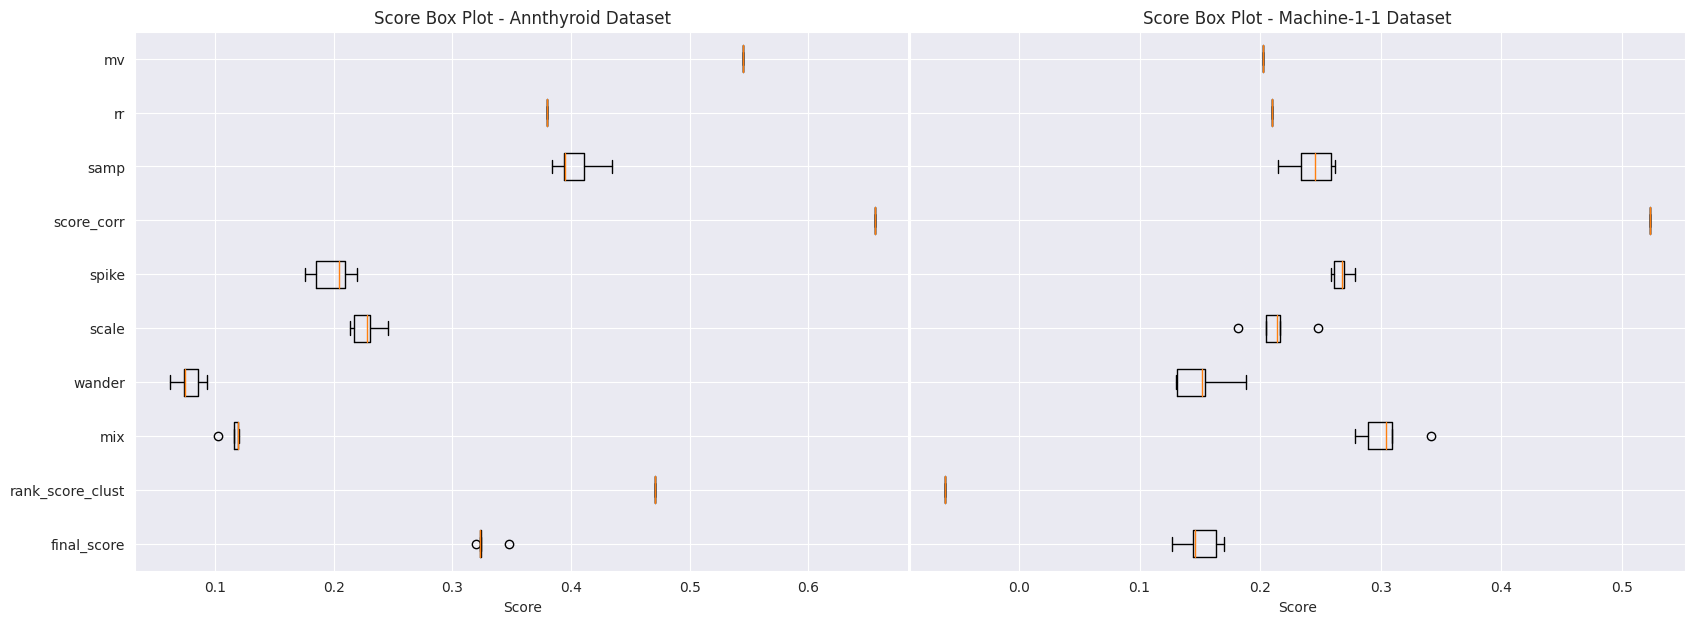
\includegraphics[width=15cm, scale=1]{images/score_box}
	\caption{Score Box Plot}
	\label{score-box}
	
\end{figure}

Queste differenze negli score vanno anche ad impattare poi il coefficiente di correlazione Kendall rispetto al Ranking Supervisionato. Anche qui, come prima, le differenze sono esigue ma sempre presenti; immagine \ref{kendall-box}.

\begin{figure}[t]
	\centering
	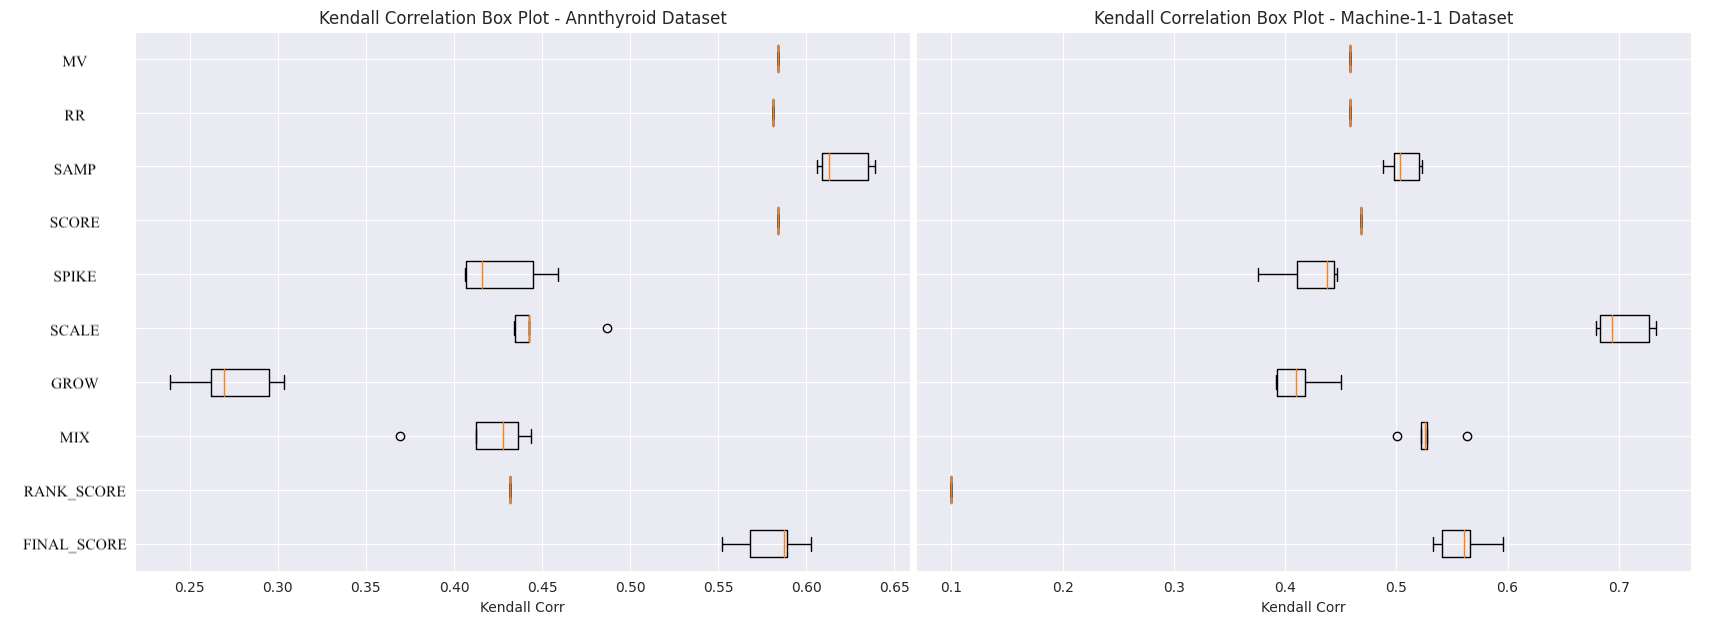
\includegraphics[width=15cm, scale=1]{images/kendall_box}
	\caption{Kendall Correlation Box Plot}
	\label{kendall-box}
		
\end{figure}


\subsubsection{Intersezione dei Quantili}
Oltre a valutare le performance sullo score di correlazione tra il ranking non supervisionato e quello supervisionato, può risultare utile cambiare punto di vista e comparare i ranking dal punto di vista dell'intersezione dei quantili.
Per questa valutazione sono stati ordinati i ranking per il loro score e poi sono stati divisi in 2 o 4 quantili. Successivamente viene calcolata l'intersezione del quantile di un ranking con il corrispondente dell'altro ranking.
Come mostrato nella figura \ref{quantile-intersection}, si può notare come dividendo in 4 quantili, l'intersezione produca uno score di circa 0.55 per i primi 3 quantili, segno che faccia più fatica nel classificare correttamente le performance dei modelli nelle posizioni più alte. Il quarto quantile però ha un punteggio di circa 0.77, segno che l'algoritmo di Model Selection sa distinguere i modelli più performanti con quelli meno performanti.

Possiamo quindi concludere che mentre il model Selection non supervisionato non sia molto preciso nel trovare il modello migliore tra quelli con performance buone, é comunque in grado di riconoscere abbastanza bene quelli peggiori. A confermare questa ipotesi il calcolo dell'intersezione dei quantili con soltanto due quantili, producendo uno score di intersezione di circa \(0.8\)

\begin{figure}[t]
	\centering
	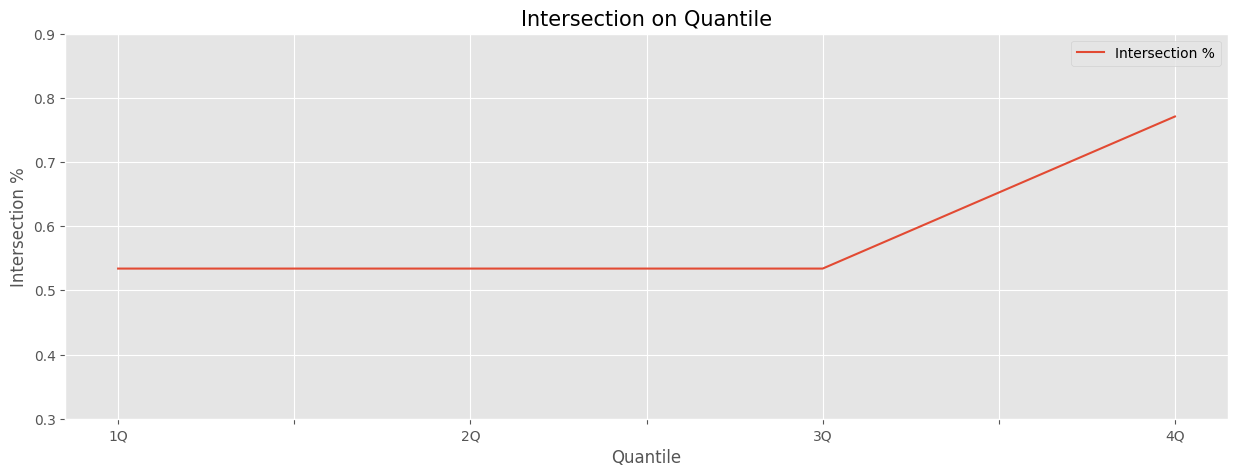
\includegraphics[width=14cm, scale=1]{images/4quantile}
	\caption{Intersezione tra quantili}
	\label{quantile-intersection}
		
\end{figure}


\newpage
\section{Risultati SKF}
Il progetto di tesi é nato da una collaborazione tra ALTEN e SKF quindi una parte dedicata a quest'ultima é necessaria. Come introdotto nel capitolo \ref{chap:skf} però, i dati prodotti dai sensori installati sui macchinari della catena di montaggio non sono sufficientemente completi per riuscire a fornire una valutazione completa dell'algoritmo di Model Selection. La mancanza di etichette e di uno storico delle manutenzioni effettuate in aggiunta al fatto che non tutte le macchine sono mappate dai sensori, rende complicato valutare i modelli di Anomaly Detection. La presenza dei dati MVM aiuta poco alla causa per tre motivi: (1) non tutte le macchine hanno sensori installati, (2) la frequenza con la quale vengono registrati i dati CoMo e troppo bassa e (3) la correlazione tra i valori dei sensori e la qualità finale non é certo da dare per scontata. Potrebbero esserci fattori aggiuntivi come la qualità del materiale utilizzato per la produzione oppure anche problemi ai macchinari che non vengono captati dai sensori. 
Nonostante ciò, viene svolta una valutazione usando MVM come riferimento. Prima viene eseguito l'algoritmo di Model Selection non supervisionato sul dataset di uno specifico macchinario andando a produrre una serie di ranking e ottenendo così il modello in prima posizione, successivamente viene usato questo per andare a fare la prediction sui dati sempre dello stesso macchinario. Infine si utilizzano i dati di MVM per:
\begin{itemize}
	\item Calcolare il numero di volte in cui un cuscinetto a sfera supera la soglia della banda A per la classe Q1 nell'intervallo di 10 minuti e paragonare questi numeri tra i time-step segnalati come anomali dal modello con i time-step segnalati come normali.
	\item Calcolare la qualità media per ogni intervallo di 10 minuti e misurare la correlazione tra la qualità con le etichette generate dal modello per ogni intervallo.
\end{itemize}
L'assunzione forte che é stata fatta é che situazione anomale di un macchinario portino a qualità del prodotto finito più bassa, ovvero a valori di MVM più alti. Quello che si spera di ottenere é vedere questa assunzione all'atto pratico, ovvero con valori di MVM mediamente più alti(qualità più bassa) per quei punti considerati anomali da un modello rispetto ai punti considerati normali.
Infine si compara il modello migliore secondo Model Selection con il modello in ultima posizione.

\subsection{Dataset}
I dataset di SKF sono stati introdotti e dettagliati nel capitolo \ref{chap:skf}. Per questa fase di valutazione vengono usati sia i dati di MVM, più nello specifico viene usata la banda A riguardante gli errori geometrici provenienti dalla fase di rettifica. Questo perché si é deciso di concentrarsi esclusivamente sul macchinario che, per motivi di privacy, chiameremo M1. Questo macchinario é il primo nella linea di produzione ed effettua la rettifica, quindi direttamente interessato alla banda A.
Per la fase di training é stato scelto il periodo che va da gennaio a marzo 2022 in quanto i dati in quel periodo risultavano i più puliti ed i più stabili da un punto di vista di oscillazioni o data-change. Mentre per la fase di prediction viene usato come riferimento il periodo maggio-giugno 2022.



\subsection{Thresholding}
Prima di procedere al training del modello é necessario avere un riferimento sulla percentuale di anomalie nel dataset. A questo scopo é stato utilizzato il metodo ${\gamma}GMM$ introdotto nel capitolo \ref{chap:methods}.
Questo algoritmo riceve in input la stessa lista di modelli candidati usati poi nel Model Selection. Dopo che i modelli sono stati allenati sul dataset di training (senza andare ad indicare il fattore di contaminazione) sono stati usati gli output score prodotti da ognuno di questi per computare la distribuzione di probabilità multivariata delle anomalie.
Il risultato prodotto da questa tecnica di thresholding é 0.05, ovvero il 5\% di punti vengono considerati anomali. Un dato ragionevole confermato dagli esperti.


\subsection{Risultati}
L'algoritmo di Model Selection, eseguito sul dataset del macchinario M1 utilizzando come modelli la medesima lista utilizzata con i dataset di benchmark, ha prodotto i seguenti risultati:


\begin{table}[H]
	\begin{minipage}{.5\textwidth}
		\centering
		\resizebox{\columnwidth}{!}{%
			\begin{tabular}{|l|l|l|l|l|l|} 
				\hline
				\textbf{\#} & \textbf{Model} & \textbf{RR} & \textbf{MIX} & \textbf{CC} & \textbf{F.Score} \\ 
				\hline
				1           & KDE            & 0.544       & 0.391        & 0.549       & 0.990            \\ 
				\hline
				2           & CBLOF\_4       & 0.539       & 0.388        & 0.501       & 0.988            \\ 
				\hline
				3           & MCD            & 0.508       & 0.483        & 0.530       & 0.955            \\ 
				\hline
				4           & IForest\_200   & 0.509       & 0.320        & 0.554       & 0.938            \\ 
				\hline
				5           & OCSVM\_poly    & 0.452       & 0.386        & 0.542       & 0.920            \\ 
				\hline
				6           & OCSVM\_sig     & 0.452       & 0.384        & 0.542       & 0.919            \\ 
				\hline
				7           & PCAODetector   & 0.552       & 1.000        & 0.510       & 0.901            \\ 
				\hline
				8           & KPCA           & 0.548       & 0.335        & 0.528       & 0.899            \\ 
				\hline
				9           & PCA            & 0.552       & 0.077        & 0.510       & 0.893            \\ 
				\hline
				10          & KNN\_10        & 0.562       & 0.286        & 0.474       & 0.830            \\
				\hline
			\end{tabular}
			}\captionof{table}{Top 10}
	\end{minipage}
	\begin{minipage}{.5\textwidth}
		\centering
		\resizebox{\columnwidth}{!}{%
			\begin{tabular}{|l|l|l|l|l|l|} 
				\hline
				\textbf{\#} & \textbf{Model} & \textbf{RR} & \textbf{MIX} & \textbf{CC} & \textbf{F.Score} \\ 
				\hline
				70          & SO\_GAAL       & 0.005       & 0.029        & 0.314       & 0.030            \\ 
				\hline
				69          & Telemanom      & 0.090       & 0.997        & 0.237       & 0.030            \\ 
				\hline
				68          & DeepSVDD       & 0.214       & 0.120        & 0.348       & 0.035            \\ 
				\hline
				67          & ALAD           & 0.071       & 0.092        & 0.375       & 0.067            \\ 
				\hline
				66          & SOS            & 0.218       & 0.143        & 0.391       & 0.098            \\ 
				\hline
				65          & SOS\_7         & 0.228       & 0.143        & 0.370       & 0.118            \\ 
				\hline
				64          & FeatureBagging & 0.335       & 0.024        & 0.406       & 0.127            \\ 
				\hline
				63          & LOF            & 0.337       & 0.065        & 0.390       & 0.136            \\ 
				\hline
				62          & PCAODetector   & 0.103       & 0.997        & 0.394       & 0.136            \\ 
				\hline
				61          & ABOD           & 0.423       & 0.054        & 0.391       & 0.139            \\
				\hline
			\end{tabular}}\captionof{table}{Worst 10}
	\end{minipage}
\end{table}




Sono proposti i primi 10 e gli ultimi 10 modelli con i relativi score finali. Le metriche surrogate utilizzate sono state (1) Round Robin per Model Centrality, (2) Mix per Performance on Injected Synthetic Anomalies e (3) Clustering Cohesion. La tecnica di aggregazione utilizzata é stato il metodo ottimale di Kemeny-Young.
Il primo modello é KDE, ovvero Kernel Density Estimation, ed in generale i metodi di Machine Learning hanno uno score più alto di quelli Deep Learning. Situazione rimarcata dal fatto che per le ultime 10 posizioni sono presenti 4 metodi di Deep Learning. Una spiegazione a questo fenomeno risiede nel fatto che questi ultimi modelli hanno score di Model Centrality e Anomaly Injection molto bassi. Eccezione per Telemanom che riesce a riconoscere quasi perfettamente tutte le anomalie sintetiche iniettate. Gli Score di Clustering Cohesion vanno anche questa volta a favorire metodi di Machine Learning, anche se in misura più lieve. Infatti i modelli come DeepSVDD o ALAD riescono a  raggiungere punteggi intorno al 0.4, in linea con i migliori.
Model Centrality va sicuramente a favorire quei modelli che producono output simile tra di loro, implicando una forte varianza dei risultati sulla base di quali modelli candidati vengono passati all'algoritmo di Model Selection. Potrebbe essere il caso che i modelli di Deep Learning siano effettivamente i migliori, ma essendo pochi rispetto al numero totale di modelli considerati, il loro punteggio di Model Centrality va abbassandosi. In questi casi, un'analisi visiva delle anomalie rilevate può risultare utile.

\subsubsection{Anomalie Rilevate}
Attraverso un grafico a linee con barre verticali per rappresentare i punti temporali rilevati come anomalia, possiamo notare nella figura \ref{kde} come KDE, ovvero il miglior modello, riesca a riconoscere bene i punti di Spike o gli intervalli di Scale in cui certi sensori raggiungono valori sufficientemente distanti da un comportamento standard. Al contrario, figura \ref{worst_clf}, Telemanom raggruppa tutti i punti anomali in un unico intervallo continuo nonostante ci siano dei punti temporali che non presentino, ad occhio, un comportamento anomalo.

\begin{figure}[t]
	\centering
	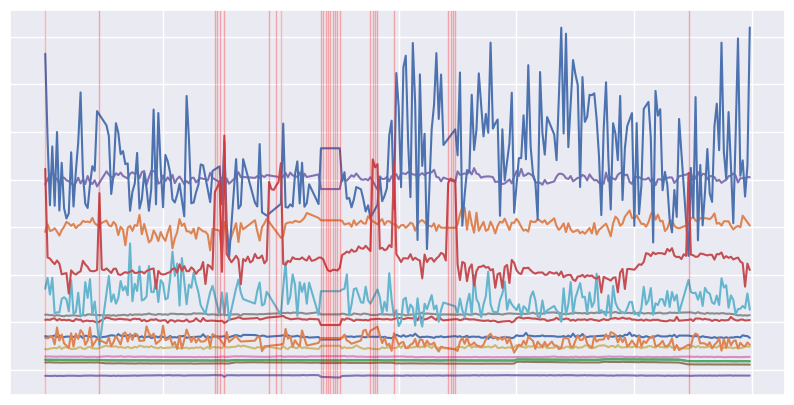
\includegraphics[width=14cm, scale=1]{images/kde}
	\caption{Anomalie Rilevate da KDE}
	\label{kde}
	
\end{figure}

\begin{figure}[t]
	\centering
	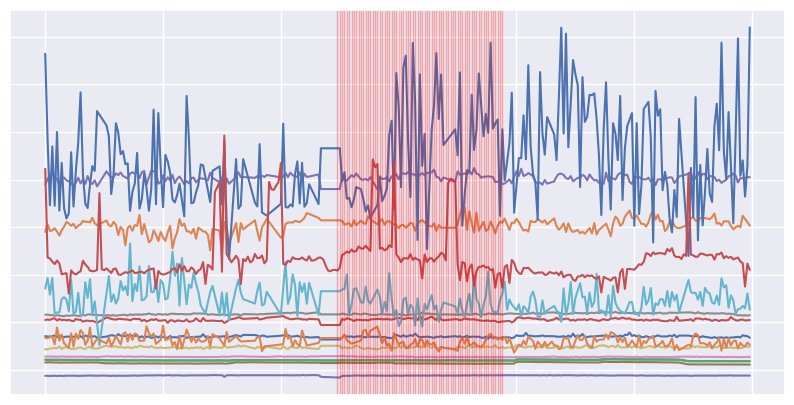
\includegraphics[width=14cm, scale=1]{images/worst_clf}
	\caption{Anomalie Rilevate da Telemanom}
	\label{worst_clf}
	
\end{figure}

Passando ad un plot scatter dopo aver ridotto la dimensionalità dei punti a 2 dimensioni tramite PCA, possiamo notare in figura \ref{kde_scatter} due cluster principali con punti sparsi nel mezzo. I punto anomali trovati da KDE si trovano principalmente nel cluster più piccolo a destra e nei punti sparsi nel piano. Mentre il cluster blu a sinistra risulta ben omogeneo.
Telemanom invece etichetta come anomali principalmente i punti all'interno del cluster di sinistra, risultando in una separazione meno chiara, figura \ref{worst_clf_scatter}.
Ovviamente non si ha la certezza che il cluster di destra sia effettivamente composto da tutti punti anomali, ma chiaramente un comportamento fuori dal normale c'è in quanto la grande maggioranza dei dati, risiedenti nel cluster di sinistra, possiedono valori molto diversi.


\begin{figure}[t]
	\centering
	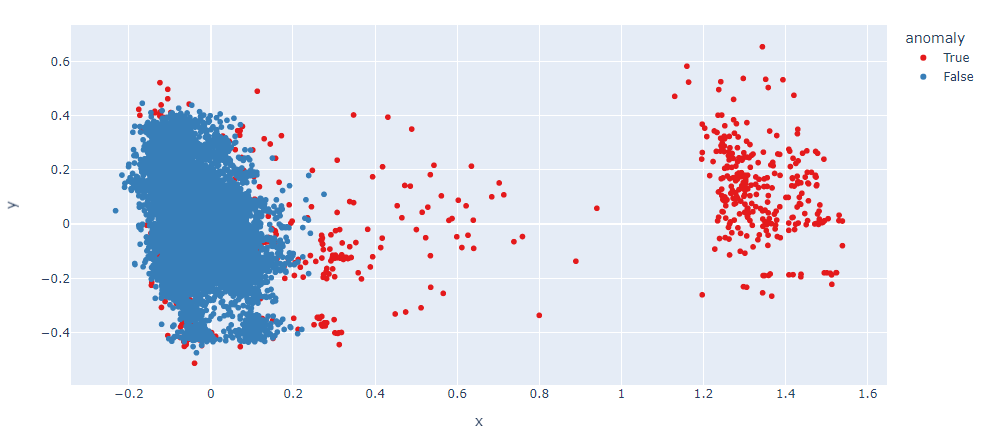
\includegraphics[width=14cm, scale=1]{images/kde_scatter}
	\caption{Scatter Plot delle anomalie KDE}
	\label{kde_scatter}
		
\end{figure}




\begin{figure}[t]
	\centering
	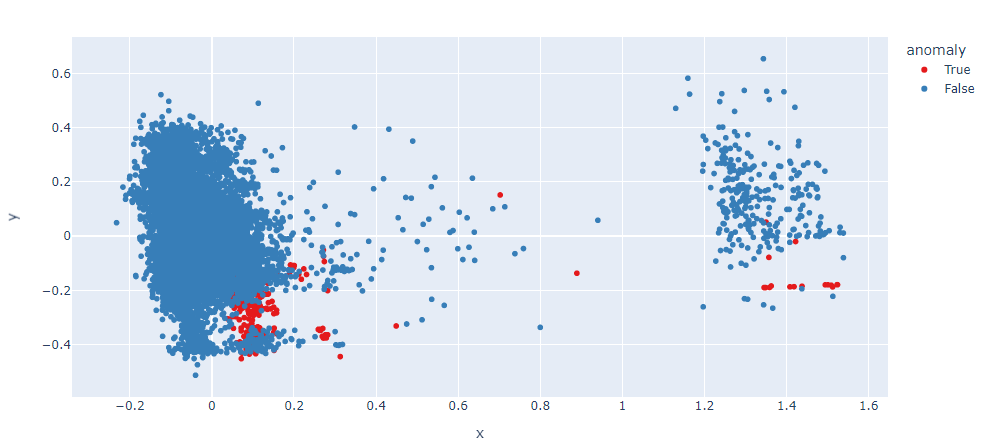
\includegraphics[width=14cm, scale=1]{images/worst_clf_scatter}
	\caption{Scatter Plot delle anomalie Telemanom}
	\label{worst_clf_scatter}
		
\end{figure}

\subsubsection{Confronto Qualità}
In questa sezione viene fatto un confronto tra le anomalie rilevate e la qualità. Come anticipato più volte, la qualità non é da considerarsi un perfetto indicatore delle anomalie: 
\begin{itemize}
	\item La qualità viene registrata ogni due secondi mentre i dati CoMo ogni 5 minuti. Di conseguenza la qualità viene aggregata con una media, andando a nascondere, nel calcolo aggregato, i valori più alti che sono anche i più rari. Usare altre tecniche di aggregazione come Min o Max non é immediato in quanto avrebbe poi favorito troppo o troppo poco la presenza di valori di qualità estremi.
	\item Analizzando un solo macchinario non é possibile avere una situazione completa della linea di produzione, ma anche analizzando tutti i macchinari insieme non é certo che la qualità sia correlata al 100\% con i dati CoMo. Ci possono essere fattori come la qualità del materiale o degli oli, o altri movimenti dei macchinari non registrati che impattano la qualità. Producendo quindi valori di qualità bassa nonostante registrazioni CoMo nella norma. Oppure il contrario, ovvero registrazioni CoMo anomale ma che non impattano la qualità.
\end{itemize}

Prima di proseguire è  necessario applicare una trasformazione hai dati. Il macchinario analizzato M1 e' il primo della linea di montaggio, mentre il macchinario di misura qualità MVM è  posto alla fine. Il cuscinetto a sfera dal momento che parte impiega un tempo ${\nabla}t$ ad arrivare ad MVM e quindi essere registrato per la misura di qualità. Per allineare quindi la registrazione CoMo di M1 con la registrazione di MVM e' necessario traslare di ${\nabla}t$ l'indice temporale della tabella MVM.

Nelle prossime due immagini possiamo vedere lo stesso scatter plot di prima, ma andando a colorare i punti sulla base della correlazione tra punti rilevati come anomali da KDE e Telemanom, e i punti registrati come bassa qualità. Le correlazioni sono così spiegate:
\begin{itemize}
	\item \textit{true positive} indica che il punto é rilevato sia come anomalo che di bassa qualità
	\item \textit{true negative} indica che il punto é rilevato sia come non anomalo che di qualità normale
	\item \textit{false negative} indica che il punto é rilevato come non anomalo ma la qualità é bassa
	\item \textit{false positive} indica che il punto é rilevato come anomalo ma la qualità é normale
\end{itemize}

L'immagine \ref{kde_quality} rappresenta lo scatter con KDE, la maggior parte dei punti del cluster di sinistra viene correttamente identificato come true-negative ma sono presenti un numero non indifferente di falsi negativi. Il cluster di destra, così come i punti sparsi nel mezzo, vengono identificati per circa metà come falsi positivi e metà come true positive.
\begin{figure}[t]
	\centering
	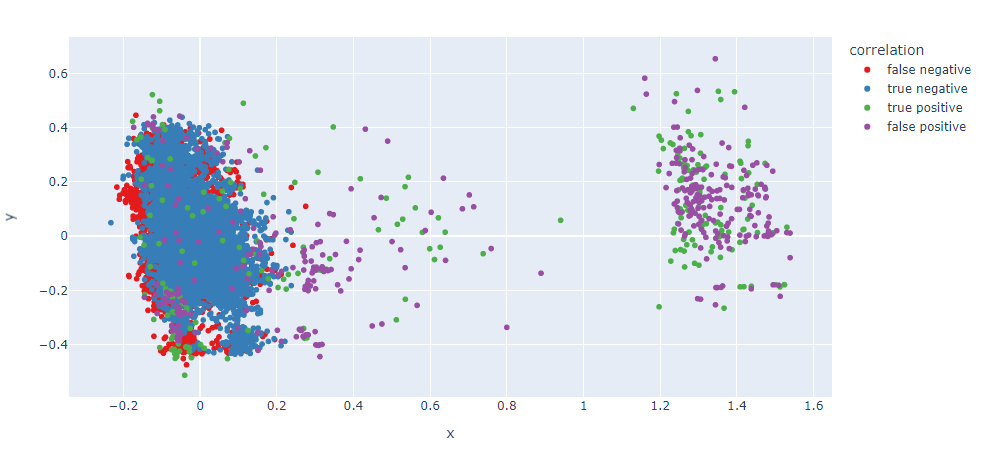
\includegraphics[width=14cm, scale=1]{images/correlation_ssb1_quality_plot.png}
	\caption{Scatter Plot Correlazione Qualità KDE}
	\label{kde_quality}
\end{figure}

Con Telemanom, immagine \ref{worst_clf_quality} la situazione non é migliore, in generale é presente confusione nell'identificazione dei punti con qualità bassa.


\begin{figure}[t]
	\centering
	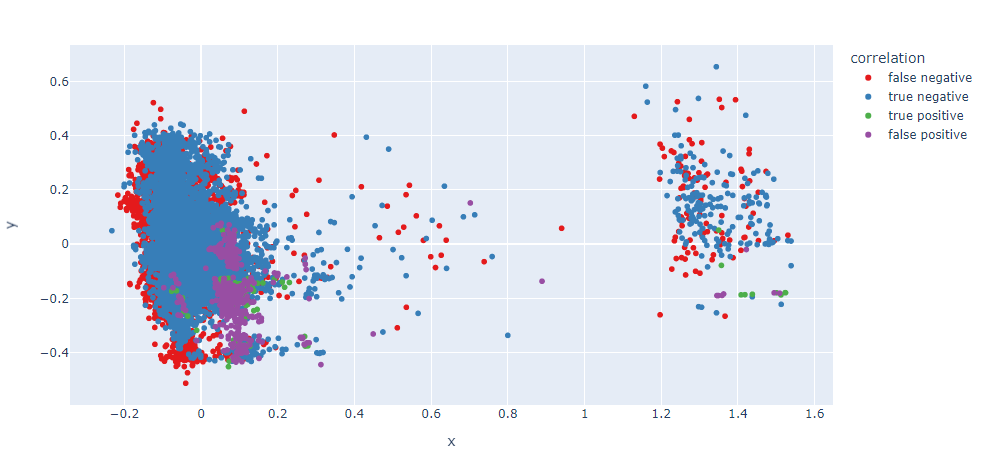
\includegraphics[width=14cm, scale=1]{images/worst_correlation_ssb1_quality_plot}
	\caption{Scatter Plot Correlazione Qualità Telemanom}
	\label{worst_clf_quality}
\end{figure}

La conferma arriva dalle matrici di confusione. Sia KDE che Telemanom non riescono a trovare punti che siano effettivamente di qualità bassa:



\begin{table}[H]
	\begin{minipage}{.5\textwidth}
		\centering
		\resizebox{\columnwidth}{!}{%
			\begin{tabular}{|l|l|l|}
				\hline
				                  & \textbf{Real Positive} & \textbf{Real Negative} \\ \hline
				\textbf{Positive} & 238 (0.05)             & 372 (0.05)             \\ \hline
				\textbf{Negative} & 4648 (0.95)            & 6885 (0.95)            \\ \hline
			\end{tabular}
			}\captionof{table}{KDE Confusion Matrix}
	\end{minipage}
	\begin{minipage}{.5\textwidth}
		\centering
		\resizebox{\columnwidth}{!}{%
			\begin{tabular}{|l|l|l|}
				\hline
				                  & \textbf{Real Positive} & \textbf{Real Negative} \\ \hline
				\textbf{Positive} & 177 (0.04)             & 430 (0.06)             \\ \hline
				\textbf{Negative} & 4709(0.96)             & 6827 (0.94)            \\ \hline
			\end{tabular}}\captionof{table}{Telemanom Confusion Matrix}
	\end{minipage}
\end{table}


\subsubsection{Confronto Qualità - Alternative}
Si potrebbe tentare di risolvere i due problemi elencati ad inizio paragrafo andando a cambiare approccio per l'analisi della correlazione.
Per il primo di questi, ovvero il problema della media di tutte le registrazioni di qualità in un dato intervallo di 10 che va a nascondere eventuali registrazioni più rare in cui la qualità é bassa, si può andare a contare il numero di registrazioni, sempre all'interno di ogni intervallo, che superano la soglia Q1 per la banda A.
I risultati ottenuti sono riportati nella tabella \ref{quality_count}.

\begin{table}[]
	\centering
	\begin{tabular}{|l|ll|ll|}
		\hline
		\multirow{2}{*}{}       & \multicolumn{2}{l|}{\textbf{Punti Normali}} & \multicolumn{2}{l|}{\textbf{Punti Anomali}} \\ \cline{2-5} 
		                        & \multicolumn{1}{l|}{Telenamom} & KDE & \multicolumn{1}{l|}{Telemanom} & KDE \\ \hline
		\textbf{Banda A}        & \multicolumn{1}{l|}{19}        & 19  & \multicolumn{1}{l|}{14}        & 19  \\ \hline
		\textbf{Tutte le bande} & \multicolumn{1}{l|}{87}        & 85  & \multicolumn{1}{l|}{72}        & 86  \\ \hline
	\end{tabular}
	\caption{\label{quality_count}Media MVM sopra-soglia per intervallo}
\end{table}

Il numero medio di registrazioni che superano la soglia Q1 della banda A all'interno degli intervalli classificati come normali da KDE sono 19, lo stesso per gli intervalli classificati come anomali. Facendo anche un conteggio tenendo in considerazione tutte le registrazione che superano la soglia Q1 di qualsiasi banda (A,B,C e D), i risultati sono 85 per i punti normali e 86 per quelli anomali. Questi risultati implicano che non c'è nessuna correlazione tra qualità bassa e punti anomali. 
Questo esperimento é stato fatto anche usando Telemanom ed anche qui i risultati confermano il trend.

Per quanto riguarda il secondo punto, ovvero il problema di considerare solamente un macchinario, si é pensato di andare a eseguire l'algoritmo di Anomaly Detection su tutti i macchinari di cui si hanno i dati della linea di produzione e aggregare insieme le etichette per ogni punto temporale.
In questo esperimento, i dati hanno bisogno di una fase di processamento aggiuntiva, ovvero é necessario allineare le registrazioni di tutti i macchinari tenendo in considerazione il tempo che impiega il cuscinetto a sfera a spostarsi lungo la linea di montaggio. In un esempio, ipotizzando tre macchine di cui la terza é MVM ed un cuscinetto a sfera che parte dalla linea di montaggio a tempo $t$, la prima macchina esegue la registrazione su quel cuscinetto a sfera a tempo $t$, la seconda a tempo $t+1$ e la terza a tempo $t+2$. Per allineare le registrazioni viene quindi rimossa un'unità temporale dalle registrazioni del secondo macchinario e 2 unità dalle registrazioni del terzo macchinario. Così facendo si crea un'istantanea delle registrazioni per ogni cuscinetto a sfera. Questo procedimento é simile a quello svolto per le valutazioni precedenti, con la differenza che in questo caso si aveva soltanto il macchinario M1 ed MVM, di conseguenza solamente i dati MVM erano da traslare.
Allineati i dati é necessario aggregare le etichette di ogni macchinario per ogni punto temporale. È stato scelto di applicare un approccio del tipo \textit{almeno uno}, ovvero se il modello di AD trova un'anomalia per un dato macchinario e per un dato punto temporale, quel punto temporale risulterà anomalo anche per tutti gli altri macchinari. 
Purtroppo però anche con questo approccio la corrispondenza tra anomalie e qualità é bassa, inoltre eseguendo l'algoritmo di AD su tutti e 10 i macchinari a disposizione e aggregando con il metodo \textit{almeno uno}, potenzialmente il numero di anomalie rilevate viene moltiplicato per 10, passando da un 5\% ad un 50\%. Questo fa lievitare i numeri di false positive a dismisura. Sia il plot scatter, figura \ref{quality_all_machines} che la matrice di confusione, tabella \ref{cm_quality_all}, sono stati posti per visualizzazione.

\begin{figure}[t]
	\centering
	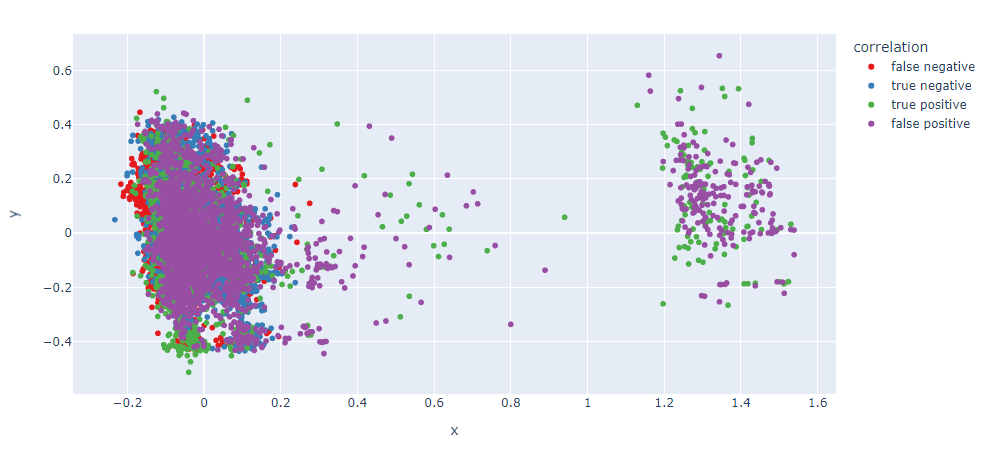
\includegraphics[width=14cm, scale=1]{images/correlation_all_quality_plot.png}
	\caption{Correlazione KDE su tutti i macchinari}
	\label{quality_all_machines}
\end{figure}

\begin{table}[]
	\centering
	\begin{tabular}{|l|l|l|}
		\hline
		                  & \textbf{Real Positive} & \textbf{Real Negative} \\ \hline
		\textbf{Positive} & 1510 (0.31)            & 2750 (0.37)            \\ \hline
		\textbf{Negative} & 3376 (0.69)            & 4507 (0.62)            \\ \hline
	\end{tabular}
	\caption{\label{cm_quality_all}Confusion Matrix KDE su tutti i macchinari}
	
\end{table}

\subsubsection{Conclusione}
In conclusione, valutare in modo automatico le performance di un modello di Anomaly Detection su SKF é di fatto impossibile. Sarebbero necessari le registrazioni di almeno tutti i macchinari della linea e frequenza di registrazione molto più alte. A questo punto un'analisi più accurata sulla relazione tra MVM e CoMo potrebbe essere svolta, ma anche in questo caso non é detto che ci sia correlazione perfetta.
L'unico modo per valutare quindi il modello prodotto da Model Selection é quello di portare in produzione una Dashboard con PowerBI, in modo da notificare gli operatori i momenti di anomalia e ricevere feedback di conseguenza sulla precisione del modello.
Una trattazione sul ciclo di distribuzione viene fatta nel capitolo successivo.